\chapter{Search for H(Inv) decays in the VBF channel with CMS parked data}
\label{CHAPTER:ParkedDataAnalysis}

\glsresetall % Resetting all acronyms

% PAS 14-038
% AN-14-243

%STATUS: DONE

The search for Higgs boson invisible decays has already been attempted in past experiments and is also the topic of many \gls{LHC} analyses. Searches were performed by the \gls{LEP} experiments \cite{ARTICLE:LEPSearchesForInvisibleHiggsBosons,ARTICLE:LEPDELPHISearchesForInvisibleDecayingHiggsBosons,ARTICLE:LEPOPALSearchForInvisiblyDecayingHiggsBosons} and at the \gls{LHC} with the full 7 and $8\,\TeV$ datasets, by the \gls{ATLAS} collaboration \cite{ARTICLE:ATLASSearchForInvisibleDecaysHiggsBosonAssociatedZ,ARTICLE:ATLASSearchForDarkMatterWithHadronicallyWorZ,ARTICLE:ATLASMonoJetPlusMET,ARTICLE:ATLASVBFHiggsInvConfNote} and by the \gls{CMS} collaboration \cite{ARTICLE:CMSVBFHiggsToInvAndZHCombination} where the most sensitive analysis was presented at chapter \ref{CHAPTER:PromptDataAnalysis}. With the assumption of the \gls{SM} production cross section and acceptance for the Higgs boson and using the \gls{VBF} production mode, the \gls{ATLAS} collaboration has placed a preliminary observed (expected) upper limit on the Higgs boson branching fraction to Invisible, \BRinv, of 0.29 (0.35) at 95\% confidence level for $m_H=125.5\,\GeV$ \cite{ARTICLE:ATLASVBFHiggsInvConfNote}. The \gls{CMS} collaboration had combined both the \gls{VBF} and ZH production modes to set an observed (expected) upper limit on the \BRinv at  $m_H=125\,\GeV$ of 0.58\,(0.44) at 95\% confidence level \cite{ARTICLE:CMSVBFHiggsToInvAndZHCombination}.

This chapter describes the analysis performed over the \gls{CMS} Run I proton-proton parked data collected over 2012. This data was recorded and stored without reconstruction and only became fully available a few months after data taking during the \gls{LS1}. The advantage of this approach was the possibility of using lower threshold triggers which can collect more signal but unfortunately also more backgrounds. To take full advantage of this data the analysis had to be redesigned and extended with new control regions. To validate the obtained results a new cross check analysis was also preformed.

%%%%%%%%%%%%%%%%%%%%%%%%%%%%%%%%%%%%%%%%%%%%%%%%%%%%%%%%%%%%%%%%%%%%%%%%%%%%%%%%%%%%
%%% SECTION
%%%%%%%%%%%%%%%%%%%%%%%%%%%%%%%%%%%%%%%%%%%%%%%%%%%%%%%%%%%%%%%%%%%%%%%%%%%%%%%%%%%%
\section{The Cross Check Analysis}
\label{CHAPTER:ParkedDataAnalysis_CrossCheckAnalysis}

%Status: DONE

It is normally a requirement for many \gls{CMS} publications to have a cross check analysis implemented independently from the main result in order to be able to ensure the accuracy of the final results due to possible errors with the software implementation. For this purpose the \gls{CMS} \gls{VBF} Higgs to invisible result using prompt data presented in chapter \ref{CHAPTER:PromptDataAnalysis}, was produced by two different and independent code frameworks. Before publication a good level of synchronization was obtained validating the obtained measurement. Due to lack of man power and time it was decide for the 2012-13 parked data analysis to only proceed with a single framework. At a later stage of the analysis it was thought that at least some level of cross check would be a good measure to limit the possibility of implementation errors and to allow extra confidence on the final results.
 
This cross check analysis starts from the physics object files, \textit{ntuples}, produced by the main analysis for all the relevant datasets. The software used for this object extraction process and its data formats are also used by other analyses at Imperial College London, including both the \gls{SM}, and \gls{MSSM} Higgs to $\tau\bar{\tau}$, the Higgs to $\tau\bar{\tau}b\bar{b}$ and prompt Higgs to invisible analyses. These analysis have been cross checked independently and therefore the part of the software is considered to be sufficiently validated. No event requirements are applied at this physics object production level except the official \gls{CMS} list of certified good luminosity sections for physics usage.
 
The analysis of these \textit{ntuples} was performed by an independent code framework which was developed in order to replicate all relevant event yields produced by the main analysis for data. Due to time constraints to the planned unbinding of the analysis, only the yields in data were cross checked.  

%%%%%%%%%%%%%%%%%%%%%%%%%%%%%%%%%%%%%%%%%%%%%%%%%%%%%%%%%%%%%%%%%%%%%%%%%%%%%%%%%%%%
%%% SECTION
%%%%%%%%%%%%%%%%%%%%%%%%%%%%%%%%%%%%%%%%%%%%%%%%%%%%%%%%%%%%%%%%%%%%%%%%%%%%%%%%%%%%
\section{Data and MC samples}

%Status: Writing

%In the analysis presented in this manuscript, the sensitivity of the CMS VBF
% analysis is improved significantly. This improvement comes from the use of a new set of
% signal selection criteria made possible by the use of triggers from the parked data 
% stream with looser thresholds than the trigger used for the previous analysis.
% The total integrated luminosity analysed is $19.2 \pm 0.5$
% fb$^{-1}$~\cite{CMS-PAS-LUM-13-001}.



%%%%%%%%%%%%%%%%%%%%%%%%%%%%%%%%%%%%%%%%%%%%%%%%%%%%%%%%%%%%%%%%%%%%%%%%%%%%%%%%%%%%
%%% SUBSECTION
%%%%%%%%%%%%%%%%%%%%%%%%%%%%%%%%%%%%%%%%%%%%%%%%%%%%%%%%%%%%%%%%%%%%%%%%%%%%%%%%%%%%
\subsection{Data}

%Status: DONE

This analysis used the full  $\sqrt{s}=8\,\TeV$ Run I proton-proton certified collision data. The total integrated luminosity analysed is $19.2 \pm 0.5 \,\femto\barn^{-1}$ \cite{ARTICLE:CMSLuminosityBasedonPixelClusterCounting}. A summary of the datasets used and their integrated luminosity can be found in table \ref{TABLE:ParkedData_Data_RunI_IntegratedLuminosity}.

\begin{table}[!htb]
\centering
\begin{tabular}{|c|c|c|}
\hline
Era & Type & $\int{Luminosity}$ $[pb^{-1}]$ \\
\hline \hline
Run A & Prompt Data &  889 \\
Run B & Parked Data & 3871 \\
Run C & Parked Data & 7152 \\
Run D & Parked Data & 7317 \\
\hline\hline
\multicolumn{2}{|c|}{Total analysed} & 19229 \\
\hline\hline
\multicolumn{2}{|c|}{Total certified luminosity} & 19789 \\
\hline
\end{tabular}
\caption{Relevant parked datasets from Run I and their total analysed integrated luminosity. Total analysed and certified also showed.}
\label{TABLE:ParkedData_Data_RunI_IntegratedLuminosity}
\end{table}


The \gls{VBF} Higgs inclusive parked trigger only became available in the beginning of the 2012 Run B. Similarly to the \textit{prompt analysis}, for Run A the prompt data recorded by the dedicated \gls{VBF} Higgs to invisible trigger is used. The difference between the certified and analysed numbers is due to the new \gls{VBF} Higgs inclusive parked trigger being present but not active for the first few runs of the 2012 Run B.

%%%%%%%%%%%%%%%%%%%%%%%%%%%%%%%%%%%%%%%%%%%%%%%%%%%%%%%%%%%%%%%%%%%%%%%%%%%%%%%%%%%%
%%% SUBSECTION
%%%%%%%%%%%%%%%%%%%%%%%%%%%%%%%%%%%%%%%%%%%%%%%%%%%%%%%%%%%%%%%%%%%%%%%%%%%%%%%%%%%%
\subsection{Monte Carlo Samples}

%Status: Writing

% \section{Simulation and object description}
% \label{sec:objects}
% 
% The analysis presented here uses the same event quality selection, definitions of physics objects and Monte Carlo (MC) samples as described in
% ~\cite{Chatrchyan:2014tja}, and summarised below.
% 
% The VBF signal is simulated using the \POWHEG 2.0 event
% generator~\cite{Nason:2004rx,Frixione:2007vw,Alioli:2009je,Hamilton:2009za,Nason:2009ai,Alioli:2010xd,Re:2010bp} hadronised with \PYTHIA 6.4.26~\cite{Sjostrand:2006za}. The
% VBF production cross sections are taken from
% ~\cite{Dittmaier:2011ti,Dittmaier:2012vm}. The main background
% processes, W and Z produced in association with jets (W/Z+jets), and
% $\ttbar$ also produced in association with jets, are
% simulated using \MADGRAPH 5.1.1~\cite{Alwall:2011uj,MadGraph} interfaced with
% \PYTHIA. For the W and Z ($\ttbar$) simulation up to 4 (3) additional partons are considered. Also for the W and Z simulation, events are generated where the W or Z boson is produced via electroweak processes as well as where they are produced via QCD processes. A VBF-topology enriched QCD multijets sample, where genuine \MET is required at generator level, has been generated with PYTHIA. Detector
% effects are then simulated using the \GEANTfour
% package~\cite{Agostinelli:2002hh,Allison:2006ve}. All MC samples are reweighted
% event-by-event to reproduce the distribution of minimum bias
% interactions (pileup) observed in data. The average number of pileup events is estimated at 21 interactions per bunch crossing.
% 
% %Additional weights are applied to simulated events to                                                                                                     
% %ensure trigger efficiency, lepton identification efficiency, and                                                                                          
% %b-tagging efficiency match measurements from data.\par}                                                                                                    
% 
% The main objects used in this analysis are jets and missing transverse energy, which are the signatures of an invisibly decaying VBF produced Higgs. Several background estimation methods used in the analysis require using control regions containing charged leptons.
% These objects are reconstructed with a particle-flow (PF)
% algorithm~\cite{CMS-PAS-PFT-09-001,CMS-PAS-PFT-10-001}. Pileup
% mitigation techniques are in place to correct the objects as well as remove objects not from the primary vertex, as
% described in detail in ~\cite{Chatrchyan:2014tja}.
% 
% Electrons~\cite{CMS:2013hoa} (muons~\cite{CMS-PAS-MUO-10-002})
% are selected in the pseudorapidity range $\abs{\eta}< 2.4 (2.1)$ and
% with p$_T> 10$\,GeV. For electrons, the $1.44 < \abs{\eta}< 1.57$
% transition region between the barrel and endcap of the electromagnetic calorimeter is excluded. Different isolation and identification criteria are used
% depending on whether the lepton is explicitly required (a tight
% lepton), where tighter criteria and p$_T> 20$\,GeV are applied, or being used for a
% veto (a veto lepton), where looser criteria and p$_T> 10$\,GeV are
% applied. A loose isolation requirement is still applied for veto
% leptons, implying that events with leptons in jets will a priori not be
% rejected. Hadronic taus are identified using the ``hadron-plus-strips''
% algorithm \cite{Chatrchyan:2012zz} which reconstructs the main
% hadronic tau decay modes using charged hadrons and photons, and leads
% to an expected efficiency of 55\% for a fake rate less than 3\%, for
% taus with p$_{T}>20$\,GeV and $|\eta|<2.3$. MC samples are reweighted
% event-by-event to match the lepton reconstruction, identification and
% isolation efficiencies measured in data.
% 
% Jets are clustered using the anti-\kt clustering
% algorithm~\cite{Cacciari:2008gp}, with a distance parameter of 0.5, as
% implemented in the \textsc{fastjet}
% package~\cite{Cacciari:fastjet1,Cacciari:fastjet2}. Jets are selected
% in the pseudorapidity range $\abs{\eta}< 4.7$ and with transverse momentum
% p$_T>30$\,GeV. Jet energy corrections are
% applied~\cite{Chatrchyan:2011ds}, as well as identification criteria
% to remove contributions from calorimeter noise or from pileup
% interactions. Jets with an identified tight electron or tight muon
% within $\Delta R < 0.5$ are filtered out.
% 
% %!!FIND ALL 4 line sentences and cut                                                                                                                  
% We define the missing transverse energy, \MET and $\phi_{\MET}$ as the
% modulus and azimuthal angle of the negative vectorial sum of the
% transverse momentum of all PF objects except the muons. Muons are
% ignored in the calculation of the \MET from trigger level onwards to
% increase the number of events in background estimation control regions
% where muons are required. Jet energy corrections (including effects
% from pileup) are propagated to the \MET object. We also use \MET significance, \METsig, defined as the ratio of the vectorial sum to the
% square root of the scalar sum of the transverse energy of all reconstructed PF
% candidates.

\begin{table}
\centering
\resizebox{0.80\linewidth}{!}{
\begin{tabular}{|l|c|c|}
\hline 
Dataset & $\sigma$ [pb] & Equivalent $\int L$ [fb$^{-1}$] \\
\hline\hline
($Z \rightarrow \nu\nu$) + jets ($50  < HT < 100   \,\GeV$) & 381.2         &    10.6 \\
($Z \rightarrow \nu\nu$) + jets ($100 < HT < 200   \,\GeV$) & 160.3         &    27.6 \\
($Z \rightarrow \nu\nu$) + jets ($200 < HT < 400   \,\GeV$) & 41.49         &     122 \\
($Z \rightarrow \nu\nu$) + jets ($400 < HT < \infty\,\GeV$) & 5.274         &     191 \\
($W \rightarrow l\nu$) + jets (inclusive)                   & 37509(NNLO)   &    2.03 \\
($W \rightarrow l\nu$) + 1 jet                              & 5400          &    42.9 \\
($W \rightarrow l\nu$) + 2 jet                              & 1750          &    19.5 \\
($W \rightarrow l\nu$) + 3 jet                              & 519           &    29.9 \\
($W \rightarrow l\nu$) + 4 jet                              & 214           &    62.5 \\
($Z/\gamma \rightarrow ll$) + jets ($M_{ll}>50\,\GeV$)      & 3503.71(NNLO) &     8.7 \\
($Z/\gamma \rightarrow ll$) + 1 jets ($M_{ll}>50\,\GeV$)    & 561           &    42.9 \\
($Z/\gamma \rightarrow ll$) + 2 jets ($M_{ll}>50\,\GeV$)    & 181           &     121 \\
($Z/\gamma \rightarrow ll$) + 3 jets ($M_{ll}>50\,\GeV$)    & 51.1          &     216 \\
($Z/\gamma \rightarrow ll$) + 4 jets ($M_{ll}>50\,\GeV$)    & 23.04         &     278 \\
EWK ($Z/\gamma \rightarrow ll$) + 2 jets                    & 0.888         &    3354 \\
EWK ($W^{+} \rightarrow l\nu$) + 2 jets                     & 6.48          &    1388 \\
EWK ($W^{-} \rightarrow l\nu$) + 2 jets                     & 4.09          &    1466 \\ 
WW                                                          & 54.838(NLO)   &     182 \\
WZ                                                          & 33.21(NLO)    &     301 \\
ZZ                                                          & 17.654(NLO)   &     555 \\
$W \gamma$                                                  & 461.6         &    10.4 \\
tt + jets                                                   & 245.8(NNLO)   &    28.2 \\
t (t-channel)                                               & 56.4(NLO)     &    66.6 \\
t (tW-channel)                                              & 11.1(NLO)     &    44.8 \\
t (s-channel)                                               & 3.79(NLO)     &    68.6 \\
$\bar{t}$ (t-channel)                                       & 30.7(NLO      &    63.0 \\
$\bar{t}$ (tW-channel)                                      & 11.1(NLO)     &    44.5 \\
$\bar{t}$ (s-channel)                                       & 1.76(NLO)     &    79.5 \\
QCD ($30  <\pt<50    \,\GeV$)                               & 66285328.0    & 0.00009 \\
QCD ($50  <\pt<80    \,\GeV$)                               & 8148778.0     & 0.00074 \\
QCD ($80  <\pt<120   \,\GeV$)                               & 1033680.0     &  0.0058 \\
QCD ($120 <\pt<170   \,\GeV$)                               & 156293.3      &   0.038 \\
QCD ($170 <\pt<300   \,\GeV$)                               & 34138.15      &   0.170 \\
QCD ($300 <\pt<470   \,\GeV$)                               & 1759.549      &    3.40 \\
QCD ($470 <\pt<600   \,\GeV$)                               & 113.8791      &    34.8 \\
QCD ($600 <\pt<800   \,\GeV$)                               & 26.9921       &     148 \\
QCD ($800 <\pt<1000  \,\GeV$)                               & 3.550036      &    1130 \\
QCD ($1000<\pt<1400  \,\GeV$)                               & 0.737844      &    1310 \\
QCD ($1400<\pt<1800  \,\GeV$)                               & 0.03352235    &   60000 \\
QCD ($1800<\pt<\infty\,\GeV$)                               & 0.001829005   &  534000 \\
\hline
\end{tabular}
}
\caption{Table of the \gls{MC} processes, corresponding cross sections (at NLO or NNLO when available) and equivalent integrated luminosity analysed.}
\label{TABLE:ParkedDataAnalysis}
\end{table}

%%%%%%%%%%%%%%%%%%%%%%%%%%%%%%%%%%%%%%%%%%%%%%%%%%%%%%%%%%%%%%%%%%%%%%%%%%%%%%%%%%%%
%%% SECTION
%%%%%%%%%%%%%%%%%%%%%%%%%%%%%%%%%%%%%%%%%%%%%%%%%%%%%%%%%%%%%%%%%%%%%%%%%%%%%%%%%%%%
\section{Monte Carlo to Data correction factors}

%Status: DONE

To correctly compare \gls{MC} with data all relevant aspects must be correctly taken into account. In the event that a variable distribution does not match between both we can determine weights to apply to each event so the distributions match again. In these analysis we apply four weights to \gls{MC}, to obtain the correct \gls{PU} distribution, weight events according to the probability of passing the trigger, account for lepton identification probability and top sample re-weghting.

%%%%%%%%%%%%%%%%%%%%%%%%%%%%%%%%%%%%%%%%%%%%%%%%%%%%%%%%%%%%%%%%%%%%%%%%%%%%%%%%%%%%
%%% SUBSECTION
%%%%%%%%%%%%%%%%%%%%%%%%%%%%%%%%%%%%%%%%%%%%%%%%%%%%%%%%%%%%%%%%%%%%%%%%%%%%%%%%%%%%
\subsection{Pile-up}

%Status: DONE?

The distribution of \gls{PU} in data and \gls{MC} simulated events samples is not the same. Each \gls{MC} dataset is re weighted event by event in order to match the observed distribution in the analysed data.

%%%%%%%%%%%%%%%%%%%%%%%%%%%%%%%%%%%%%%%%%%%%%%%%%%%%%%%%%%%%%%%%%%%%%%%%%%%%%%%%%%%%
%%% SUBSECTION
%%%%%%%%%%%%%%%%%%%%%%%%%%%%%%%%%%%%%%%%%%%%%%%%%%%%%%%%%%%%%%%%%%%%%%%%%%%%%%%%%%%%
\subsection{Trigger efficiency}
\label{SUBSECTION:ParkedDataAnalysis_CorrectionFactors_TriggerEfficiency}

% \section{Triggering and selection}
% \label{sec:sel}
% The same analysis strategy as in ~\cite{Chatrchyan:2014tja} is
% used. The pair of jets from VBF production have the distinct topology
% of being well separated in $\eta$, in opposite forward/backward halves
% of the detector, and having a high dijet invariant mass,
% M$_{jj}$. Final states with the two highest p$_{T}$ two jets with this VBF topology and large
% missing transverse energy are therefore selected.
% 
% The triggers available during 2012 varied across different data-taking
% periods. For each period (named A, B, C and D) the unprescaled
% VBF-specific trigger with the loosest selection criteria is used, this
% leads to three different triggers being used in total. At the first trigger level (L1T) used by CMS all three have the same selection, requiring L1T \MET$>40$\,GeV, which is the \MET calculated using calorimeter trigger towers with $|\eta|<3$. The trigger used
% in run A is the same as the prompt trigger used in
% Ref.~\cite{Chatrchyan:2008aa}, and selects, among all possible jet
% pairs to minimise the impact of pileup, at least one pair of PF jets
% with p$_T>40$\,GeV, M$_{jj}>800$\,GeV, dijet
% pseudorapidity difference $\Delta\eta_{jj}>3.5$ and $\MET>65$\,GeV. The integrated
% luminosity for run A is $0.89 \pm 0.02$\,fb$^{-1}$. The trigger used
% for run B and C (D) is a parked trigger that selects a pair of
% calorimeter jets with p$_T>35 (30)$\,GeV, M$_{jj}>700$\,GeV and
% $\Delta\eta_{jj}>3.5$. The integrated luminosity for runs B and C (D)
% is $11.0 \pm 0.3$ ($7.3 \pm 0.2$)\,fb$^{-1}$. To take into account the
% correlations between the different variables, the efficiency of each
% trigger is measured as a function of \MET in bins of M$_{jj}$ and
% sub-leading jet p$_{T}$, using independent events recorded by a
% single-muon trigger. All MC samples are then weighted event-by-event
% by the luminosity-weighted average of the three measured efficiencies.
% 
% The data recorded by the triggers is dominated by QCD multijet
% events. Multijet events have two distinct origins: (1) events with
% fake \MET, where the \MET comes from mismeasured jets in the events;
% and (2) events with genuine \MET, where the \MET comes from the decay
% of hadrons involving neutrinos, in particular heavy-flavour
% decays. The fake \MET contribution can be reduced by requiring \METsig 
% to be large. Both components can be reduced by isolating
% the \MET, by requiring that the minimum azimuthal angle separation
% between any reconstructed jet with p$_T>30$ GeV and the \MET,
% \mindphiall, be large.
% 
% The trigger requirements together with the need to reduce the QCD multijet
% contribution to negligible levels drive the choice of the following
% selection criteria:
% 
% \begin{equation}
%   \label{eq:sel}
%   \begin{aligned}
%     &\eta_{j1} \cdot \eta_{j2}<0,\, \eta_{j1}<4.7,\, \eta_{j2}<4.7,\\
%     &p_{T}^{\text{j1}}>50 \,\text{GeV},\,p_{T}^{\text{j2}}>40\,\text{GeV},\\
%     &\Delta\eta_{jj}>3.6,\, M_{jj}>1000\,\text{GeV}, \\
%     &\MET>90\,\text{GeV},\\
%     & \mindphiall > 2.0,\,\METsig>4.
%   \end{aligned}
% \end{equation}
% 
% where j1 and j2 are the two leading jets ordered by decreasing p$_T$.  In
% addition, the selected events are required to have no electrons or muons fulfilling the veto identification criteria (as defined in Sec. \ref{sec:objects}).
% 
% At this stage in the selection, the background processes leading to a
% similar final state are, by order of decreasing importance:
% W($\ell\nu$) and Z($\nu\nu$) + jets, QCD multijet production, all top
% channels (\ttbar and single top channels), dibosons, and
% Drell--Yan$(\ell\ell)\text{+jets}$. The selection is further optimised
% by tightening the requirements listed above to find the best 95\%
% C.L. expected limit on \BRinv for a \mH=125 GeV Higgs boson.  The
% optimal additional selection is found to be $\mindphiall > 2.3$,
% p$_{T}^{j2}>45$\,GeV and M$_{jj}>1200$\,GeV, and these requirements
% along with those in Eq.~\ref{eq:sel} are used to define the signal
% region.

%Status: DONE

The initial event selection for this analysis starts with a dedicated set of triggers which were recorded to the \gls{VBF} parked dataset. We used the following \gls{HLT} trigger paths for each Run I era:

\begin{itemize}
  \item Run A:       \verb!HLT_DiPFJet40_PFMETnoMu65_MJJ800VBF_AllJets!
  \item Run B and C: \verb!HLT_DiJet35_MJJ700_AllJets_DEta3p5_VBF!
  \item Run D:       \verb!HLT_DiJet30_MJJ700_AllJets_DEta3p5!
\end{itemize}

All the used paths are seeded by \gls{L1T} trigger condition \verb!L1_ETM40!. 

To maximize the usage of the event statistics of the selected \gls{MC} samples, we do not veto events that fail the trigger conditions. Instead an event by event weight is calculated which which taking into account how much luminosity was recorded by each of the three trigger and depending on the offline quantities which correspond to the ones used in the trigger conditions: PFMETnoMu, leading dijet $m_{jj}$ and sub-leading jet \pt. 

To define the weights, turn on curves were determined according to these offline variables as a function of PFMETnoMu in bins of dijet $m_{jj}$ and sub-leading jet \pt. This approach allows the determination of the weights which include the correlations between these variables. The turn on curves are obtained by fitting equation \ref{EQUATION:ParkedDataAnalysis_TriggerEfficiency_Efficiency} to each bin.

\begin{equation}
\frac{\varepsilon_{max}}{2}\text{Erf}\left(\frac{x-x_{0}}{\sqrt{\Gamma}}\right)+1,
\label{EQUATION:ParkedDataAnalysis_TriggerEfficiency_Efficiency} 
\end{equation}

Where $\varepsilon_{max}$ os the maximum efficiency of the trigger in the bin, $x_{0}$ is the mid-value of the turn on and $\Gamma$ is the width of the turn on.

%%%%%%%%%%%%%%%%%%%%%%%%%%%%%%%%%%%%%%%%%%%%%%%%%%%%%%%%%%%%%%%%%%%%%%%%%%%%%%%%%%%%
%%% SUBSECTION
%%%%%%%%%%%%%%%%%%%%%%%%%%%%%%%%%%%%%%%%%%%%%%%%%%%%%%%%%%%%%%%%%%%%%%%%%%%%%%%%%%%%
\subsection{Lepton Identification}

%Status: Writing

%%%%%%%%%%%%%%%%%%%%%%%%%%%%%%%%%%%%%%%%%%%%%%%%%%%%%%%%%%%%%%%%%%%%%%%%%%%%%%%%%%%%
%%% SUBSECTION
%%%%%%%%%%%%%%%%%%%%%%%%%%%%%%%%%%%%%%%%%%%%%%%%%%%%%%%%%%%%%%%%%%%%%%%%%%%%%%%%%%%%
\subsection{Top reweighting}

%Status: Writing

%%%%%%%%%%%%%%%%%%%%%%%%%%%%%%%%%%%%%%%%%%%%%%%%%%%%%%%%%%%%%%%%%%%%%%%%%%%%%%%%%%%%
%%% SECTION
%%%%%%%%%%%%%%%%%%%%%%%%%%%%%%%%%%%%%%%%%%%%%%%%%%%%%%%%%%%%%%%%%%%%%%%%%%%%%%%%%%%%
\section{Signal event selection}
\label{SECTION:ParkedDataAnalysis_SignalEventSelection}

%Status: Writing

\begin{table}[!htp]
\centering
\begin{tabular}{|l|c|c|c|c||c|}
\hline
 & \rotatebox{90}{Prompt Run A} & \rotatebox{90}{Parked Run B} & \rotatebox{90}{Parked Run C} & \rotatebox{90}{Parked Run D} & \rotatebox{90}{Total Data} \\
\hline \hline
Vertex Filter                   & 3606391 & 132346320 & 228049748 & 308041846 & 672044305 \\
Event Quality Filters           & 2658960 & 131554431 & 226680352 & 305918529 & 666812272 \\
ECAL Laser Filter               & 2634271 & 131543040 & 226680352 & 305918529 & 666776192 \\
HCAL Laser Filter               & 2634080 & 131543040 & 226679741 & 305918529 & 666775390 \\
L1T ETM Filter                  & 2461217 &  88174347 & 160560859 & 227801622 & 478998045 \\
HLT Filter                      &   97522 &  75100422 & 137527238 & 152041761 & 364766943 \\
$N(Electrons_{veto})=0$         &   96600 &  74947192 & 137241812 & 151725585 & 364011189 \\
$N(Muon_{loose})=0$             &   94864 &  74913002 & 137179173 & 151652654 & 363839693 \\
Dijet cut                       &   18338 &  13678405 &  25090291 &  24082304 &  62869338 \\
MET cut                         &    4167 &     38178 &     68047 &     79723 &    190115 \\
$MET_{Significance}$ cut        &     786 &      3396 &      5988 &      5567 &     15737 \\
$Min(\Delta\phi(MET,jets))$ cut &      34 &        91 &       205 &       178 &       508 \\
\hline
\end{tabular}
\caption{Table of the step by step event yield for the signal region obtained by the cross check analysis section.}
\label{TABLE:ParkedDataAnalysis_SignalEventSelection_CrossSectionYields}
\end{table}



%%%%%%%%%%%%%%%%%%%%%%%%%%%%%%%%%%%%%%%%%%%%%%%%%%%%%%%%%%%%%%%%%%%%%%%%%%%%%%%%%%%%
%%% SECTION
%%%%%%%%%%%%%%%%%%%%%%%%%%%%%%%%%%%%%%%%%%%%%%%%%%%%%%%%%%%%%%%%%%%%%%%%%%%%%%%%%%%%
\section{Control Regions}

%Status: Writing

%%%%%%%%%%%%%%%%%%%%%%%%%%%%%%%%%%%%%%%%%%%%%%%%%%%%%%%%%%%%%%%%%%%%%%%%%%%%%%%%%%%%
%%% SUBSECTION
%%%%%%%%%%%%%%%%%%%%%%%%%%%%%%%%%%%%%%%%%%%%%%%%%%%%%%%%%%%%%%%%%%%%%%%%%%%%%%%%%%%%
\subsection{Top background estimation}

%Status: Writing

%%%%%%%%%%%%%%%%%%%%%%%%%%%%%%%%%%%%%%%%%%%%%%%%%%%%%%%%%%%%%%%%%%%%%%%%%%%%%%%%%%%%
%%% SUBSECTION
%%%%%%%%%%%%%%%%%%%%%%%%%%%%%%%%%%%%%%%%%%%%%%%%%%%%%%%%%%%%%%%%%%%%%%%%%%%%%%%%%%%%
\subsection{W background estimation}

%Status: Writing

%%%%%%%%%%%%%%%%%%%%%%%%%%%%%%%%%%%%%%%%%%%%%%%%%%%%%%%%%%%%%%%%%%%%%%%%%%%%%%%%%%%%
%%% SUBSECTION
%%%%%%%%%%%%%%%%%%%%%%%%%%%%%%%%%%%%%%%%%%%%%%%%%%%%%%%%%%%%%%%%%%%%%%%%%%%%%%%%%%%%
\subsection{W background estimation}

%Status: Writing

%%%%%%%%%%%%%%%%%%%%%%%%%%%%%%%%%%%%%%%%%%%%%%%%%%%%%%%%%%%%%%%%%%%%%%%%%%%%%%%%%%%%
%%% SUBSUBSECTION
%%%%%%%%%%%%%%%%%%%%%%%%%%%%%%%%%%%%%%%%%%%%%%%%%%%%%%%%%%%%%%%%%%%%%%%%%%%%%%%%%%%%
\subsubsection{W to electron+neutrino}

%Status: Writing

%%%%%%%%%%%%%%%%%%%%%%%%%%%%%%%%%%%%%%%%%%%%%%%%%%%%%%%%%%%%%%%%%%%%%%%%%%%%%%%%%%%%
%%% SUBSUBSECTION
%%%%%%%%%%%%%%%%%%%%%%%%%%%%%%%%%%%%%%%%%%%%%%%%%%%%%%%%%%%%%%%%%%%%%%%%%%%%%%%%%%%%
\subsubsection{W to muon+neutrino}

%Status: Writing

%%%%%%%%%%%%%%%%%%%%%%%%%%%%%%%%%%%%%%%%%%%%%%%%%%%%%%%%%%%%%%%%%%%%%%%%%%%%%%%%%%%%
%%% SUBSUBSECTION
%%%%%%%%%%%%%%%%%%%%%%%%%%%%%%%%%%%%%%%%%%%%%%%%%%%%%%%%%%%%%%%%%%%%%%%%%%%%%%%%%%%%
\subsubsection{W to tau+neutrino}

%Status: Writing

%%%%%%%%%%%%%%%%%%%%%%%%%%%%%%%%%%%%%%%%%%%%%%%%%%%%%%%%%%%%%%%%%%%%%%%%%%%%%%%%%%%%
%%% SUBSECTION
%%%%%%%%%%%%%%%%%%%%%%%%%%%%%%%%%%%%%%%%%%%%%%%%%%%%%%%%%%%%%%%%%%%%%%%%%%%%%%%%%%%%
\subsection{Z background estimation}

%Status: Writing

%%%%%%%%%%%%%%%%%%%%%%%%%%%%%%%%%%%%%%%%%%%%%%%%%%%%%%%%%%%%%%%%%%%%%%%%%%%%%%%%%%%%
%%% SUBSECTION
%%%%%%%%%%%%%%%%%%%%%%%%%%%%%%%%%%%%%%%%%%%%%%%%%%%%%%%%%%%%%%%%%%%%%%%%%%%%%%%%%%%%
\subsection{QCD background estimation}

%Status: Writing

%%%%%%%%%%%%%%%%%%%%%%%%%%%%%%%%%%%%%%%%%%%%%%%%%%%%%%%%%%%%%%%%%%%%%%%%%%%%%%%%%%%%
%%% SUBSUBSECTION
%%%%%%%%%%%%%%%%%%%%%%%%%%%%%%%%%%%%%%%%%%%%%%%%%%%%%%%%%%%%%%%%%%%%%%%%%%%%%%%%%%%%
\subsubsection{QDC VBF-like + MET Monte Carlo Sample}

%Status: Writing

%%%%%%%%%%%%%%%%%%%%%%%%%%%%%%%%%%%%%%%%%%%%%%%%%%%%%%%%%%%%%%%%%%%%%%%%%%%%%%%%%%%%
%%% SUBSUBSECTION
%%%%%%%%%%%%%%%%%%%%%%%%%%%%%%%%%%%%%%%%%%%%%%%%%%%%%%%%%%%%%%%%%%%%%%%%%%%%%%%%%%%%
\subsubsection{Data driven QCD estimation}

%Status: Writing

%%%%%%%%%%%%%%%%%%%%%%%%%%%%%%%%%%%%%%%%%%%%%%%%%%%%%%%%%%%%%%%%%%%%%%%%%%%%%%%%%%%%
%%% SECTION
%%%%%%%%%%%%%%%%%%%%%%%%%%%%%%%%%%%%%%%%%%%%%%%%%%%%%%%%%%%%%%%%%%%%%%%%%%%%%%%%%%%%
\section{Systematics}

%Status: DONE

The dominant source of uncertainty is due to the statistical uncertainty associated with the yields of the control regions both in data and \gls{MC} simulation, which are used for the estimation of the different backgrounds in signal region. 

The errors associated to the jet energy scale, unclustered energy scale and jet energy resolution are estimated for both signal and background processes by varying each quantity independently by its uncertainties \cite{ARTICLE:CMSDeterminationJetEnergyCalibration}. For each variation the \gls{MET} is recomputed and the signal and backgrounds predictions are recalculated. A similar procedure is applied for the lepton efficiency and \gls{PU} scale factors which are applied to the \gls{MC} simulation, which are also varied by their uncertainties and propagated through the analysis \cite{ARTICLE:CMSMuonReconstruction7TeV,ARTICLE:CMSElectronReconstruction8TeV}.

The uncertainty associated with the integrated luminosity measurement is of 2.6\% and is only applied to the \gls{MC} simulated signal and backgrounds \cite{ARTICLE:CMSLuminosityBasedonPixelClusterCounting}. The main backgrounds are normalised using a data-driven method which takes into account the trigger efficiency, while the impact of the luminosity measurement in the signal and minor backgrounds was found to be negligible.

Uncertainties associated with diboson cross sections are taken from \gls{CMS} measurements \cite{ARTICLE:CMSMeasurmentOfWWandZZxsec}, while the theoretical uncertainties due to \gls{PDF} and \gls{QCD} scales associated to the signal cross section are taken from the \gls{LHC} Higgs Cross Section Working Groups Yellow Report 3 \cite{ARTICLE:HandbookofLHCHiggsCrossSectionsInclusiveObservables,ARTICLE:HandbookofLHCHiggsCrossSectionsDifferentialDistributions}.

% TODO: Ask patrick, ``compatible within statistical uncertainty`` of what?
The uncertainty of the extrapolation of the  $Z\rightarrow\nu\nu$ background obtained from the \gls{QCD} production of $Z/\gamma^{*}\rightarrow\mu\mu$ was estimated by comparing the prediction from \textsc{MADGRAPH} and a\textsc{MC@NLO\_MG5} \cite{ARTICLE:aMCatNLO}. The results from both generators were compatible within statistical uncertainty, leading to no additional uncertainties being added. 

Table \ref{TABLE:ParkedDataAnalysis_Systematics_Summary} shows a summary of the overall size of each uncertainty as a percentage of the total signal and background predictions.

\begin{table}[!htb]
\centering
\begin{tabular}{|l|c|c|}
\hline 
Source                                            & Total background &     Signal \\
\hline\hline
Control region data stat.                          &            9.3  &          - \\
MC stat.                                           &            5.4  &        3.8 \\
Jet energy scale                                   &            4.6  &         11 \\
$W\rightarrow\tau\nu$ control region extrapolation &            4.3  &          - \\
QCD normalisation                                  &            3.2  &          - \\
Jet energy resolution                              &            3.0  &        1.8 \\
Lepton ID efficiency                               &            2.4  &          - \\
Unclustered energy scale                           &            1.9  &        1.6 \\
Pileup weight                                      &            1.1  &        1.5 \\
Top MC scale factor unc.                           &            0.25 &          - \\
Luminosity                                         &            0.02 &        2.6 \\
QCD scale, PDF and cross section uncertainties     &            0.01 &        5.2 \\
\hline
\end{tabular}
\caption{Summary of the uncertainties on the total background and signal yields. All uncertainties affect the normalization of the yield, and are quoted as the change in \% in the total background or signal estimate, when each systematic effect is varied according to its uncertainties. The signal uncertainties are given for $m_H=125$\GeV and $\BRinv=100$\%. \cite{ARTICLE:CMSVBFHiggsInvisibleParkedAnalysisPAS}}
\label{TABLE:ParkedDataAnalysis_Systematics_Summary}
\end{table}

%%%%%%%%%%%%%%%%%%%%%%%%%%%%%%%%%%%%%%%%%%%%%%%%%%%%%%%%%%%%%%%%%%%%%%%%%%%%%%%%%%%%
%%% SECTION
%%%%%%%%%%%%%%%%%%%%%%%%%%%%%%%%%%%%%%%%%%%%%%%%%%%%%%%%%%%%%%%%%%%%%%%%%%%%%%%%%%%%
\section{Results}

%Status: Writing

\begin{table}[!htb]
\centering
\begin{tabular}{|l|c|}
\hline 
Process & Event yields \\
\hline\hline
$Z\rightarrow\nu\nu$  & $158.1 \pm 37.3 \pm 21.2$ \\
$W\rightarrow\mu\nu$  & $102.5 \pm 6.2  \pm 11.7$ \\
$W\rightarrow e\nu$   & $ 57.9 \pm 7.4  \pm  7.7$ \\
$W\rightarrow\tau\nu$ & $ 94.6 \pm 13.1 \pm 23.8$ \\
top                   & $  5.5 \pm 1.8$           \\
VV                    & $  3.9 \pm 0.7$           \\
QCD multijet          & $ 17   \pm 14$            \\
\hline\hline
Total Background      & $439.4 \pm 40.7 \pm 43.5$ \\
\hline\hline
Signal(VBF)           & $273.1 \pm 31.2 $         \\
Signal(ggH)           & $ 23.1 \pm 15.9 $         \\
\hline\hline
Observed data         & 508                       \\
\hline
\end{tabular}
\caption{TODO \cite{ARTICLE:CMSVBFHiggsInvisibleParkedAnalysisPAS}}
\label{TABLE:ParkedDataAnalysis_Results_Summary}
\end{table}

\subsection{Comparison with the cross-check analysis}

%Status: Writing

\begin{table}[!htb]
\centering
\begin{tabular}{|l|c|c|c|}
\hline
Region                & Main & Cross Check & Difference [\%] \\
\hline\hline
$Z\rightarrow\nu\nu$  &   18 &          18 &             0.0 \\
$W\rightarrow\mu\nu$  &  300 &         300 &             0.0 \\
$W\rightarrow e\nu$   &   68 &          68 &             0.0 \\
$W\rightarrow\tau\nu$ &   76 &          76 &             0.0 \\
top                   &   21 &          21 &             0.0 \\
QCD Norm1             & 1586 &        1603 &            +1.1 \\
QCD Norm2             &  411 &         412 &            +0.2 \\
QCD Norm3             & 1517 &        1523 &            +0.4 \\
\hline\hline
Signal                &  508 &         508 &             0.0 \\
\hline
\end{tabular}
\caption{TODO}
\label{TABLE:ParkedDataAnalysis_Results_MainCrossCheckComparison}
\end{table}



%%%%%%%%%%%%%%%%%%%%%%%%%%%%%%%%%%%%%%%%%%%%%%%%%%%%%%%%%%%%%%%%%%%%%%%%%%%%%%%%%%%%
%%% SECTION
%%%%%%%%%%%%%%%%%%%%%%%%%%%%%%%%%%%%%%%%%%%%%%%%%%%%%%%%%%%%%%%%%%%%%%%%%%%%%%%%%%%%
\section{Extraction of limits}

%Status: Writing

\begin{figure}[h!]
  \begin{center}
    \includegraphics[width=0.49\textwidth]{Chapter07/Images/vbflimit.pdf} %!!UNBLIND ALREADY IN                                                                       
    \includegraphics[width=0.49\textwidth]{Chapter07/Images/vbfxslimit.pdf}
 \caption{The 95\% C.L. limit on \BRinv\, of a SM Higgs
boson (left) and the 95\% C.L. limit on the cross section times
\BRinv\, (right)as a function of the Higgs
boson mass, assuming SM Higgs boson acceptances. \cite{ARTICLE:CMSVBFHiggsInvisibleParkedAnalysisPAS}}
    \label{fig:limits}
  \end{center}
\end{figure}


%%%%%%%%%%%%%%%%%%%%%%%%%%%%%%%%%%%%%%%%%%%%%%%%%%%%%%%%%%%%%%%%%%%%%%%%%%%%%%%%%%%%
%%% SECTION
%%%%%%%%%%%%%%%%%%%%%%%%%%%%%%%%%%%%%%%%%%%%%%%%%%%%%%%%%%%%%%%%%%%%%%%%%%%%%%%%%%%%
\section{Summary}
\label{SECTION:ParkedDataAnalysis_Summary}



%%%%%%%%%%%%%%%%%%%%%%%%%%%%%%%%%%%%%%%%%%%%%%%%%%%%%%%%%%%%%%%%%%%%%%%%%%%%%%%%%%%%
%%%%%%%%%%%%%%%%%%%%%%%%%%%%%%%%%%%%%%%%%%%%%%%%%%%%%%%%%%%%%%%%%%%%%%%%%%%%%%%%%%%%
%%%%%%%%%%%%%%%%%%%%%%%%%%%%%%%%%%%%%%%%%%%%%%%%%%%%%%%%%%%%%%%%%%%%%%%%%%%%%%%%%%%%
%%%%%%%%%%%%%%%%%%%%%%%%%%%%%%%%%%%%%%%%%%%%%%%%%%%%%%%%%%%%%%%%%%%%%%%%%%%%%%%%%%%%
% 
% 

%
%%%%%%%%%%%
%
% \section{Background Estimation}
% \label{sec:bkg}
% The major W and Z backgrounds are estimated using MC normalised to the
% data in independent control regions, described below. The QCD
% background is estimated from data. The contributions from other minor
% backgrounds, \ie top, dibosons and Drell Yan, are taken directly from MC.
% 
% The contribution to the signal region from the Z($\nu\nu$)+jets process is normalised
% using visible Z$\rightarrow\mu\mu$ decays as a control region. The control
% region is defined as the region satisfying the same selection as the signal region,
%  except that the lepton veto is replaced with a requirement that the only leptons present in the event
% are a pair of oppositely charged tight muons with their invariant mass, $M_{\mu\mu}$, between
% 60 and 120 GeV. The number of Z($\nu\nu$) events in the
% signal region is then taken to be:
% 
% \begin{equation}
%   \label{eq:mumueq}
%   N_{S}^{Z\rightarrow\nu\nu}=\left(N_{C}^{Data}-N_{C}^{bkg}\right) \cdot\frac{\sigma\left(Z\rightarrow\nu\nu\right)}{\sigma\left(Z/\gamma^{*}\rightarrow\mu\mu\right)}\cdot \frac{\epsilon_{S}^{ZMC}}{\epsilon_{C}^{ZMC}},
% \end{equation}
% 
% where the ratio of cross-sections
% $\sigma(Z\rightarrow\nu\nu)$/$\sigma(Z/\gamma^{*}\rightarrow\mu\mu)=5.651\pm
% 0.023$ \syst, $\epsilon_{S}^{ZMC}=(1.8\pm 0.1)\cdot 10^{-6}$ and $\epsilon_{C}^{ZMC}=(1.2\pm 0.1)\cdot 10^{-6}$ are the efficiency of the selection in the signal and control regions respectively, $N_{C}^{Data}=18\pm 4.2$ is the number of data events in the control region, and $N_{C}^{bkg}=0.2 \pm 0.1 \stat$ is the number of
% events from other processes leading to the $\mu\mu$ final state estimated from MC simulation. The
% contribution from electroweak produced Z+jets events to the final estimate is
% 21\%. Distributions of the pseudorapidity of the two leading jets,
% M$_{jj}$, \METsig and \MET are shown in Fig.~\ref{fig:mumucontplots}. Within
% the statistics available, a good agreement between data and MC is
% observed. The final estimate of the $Z\rightarrow \nu\nu$ background
% is $N_{S}^{Z\rightarrow\nu\nu}= 158.1 \pm 37.8 \stat \pm 21.2
% \syst$.
% 
% \begin{figure}[h!]
%   \begin{center}
%     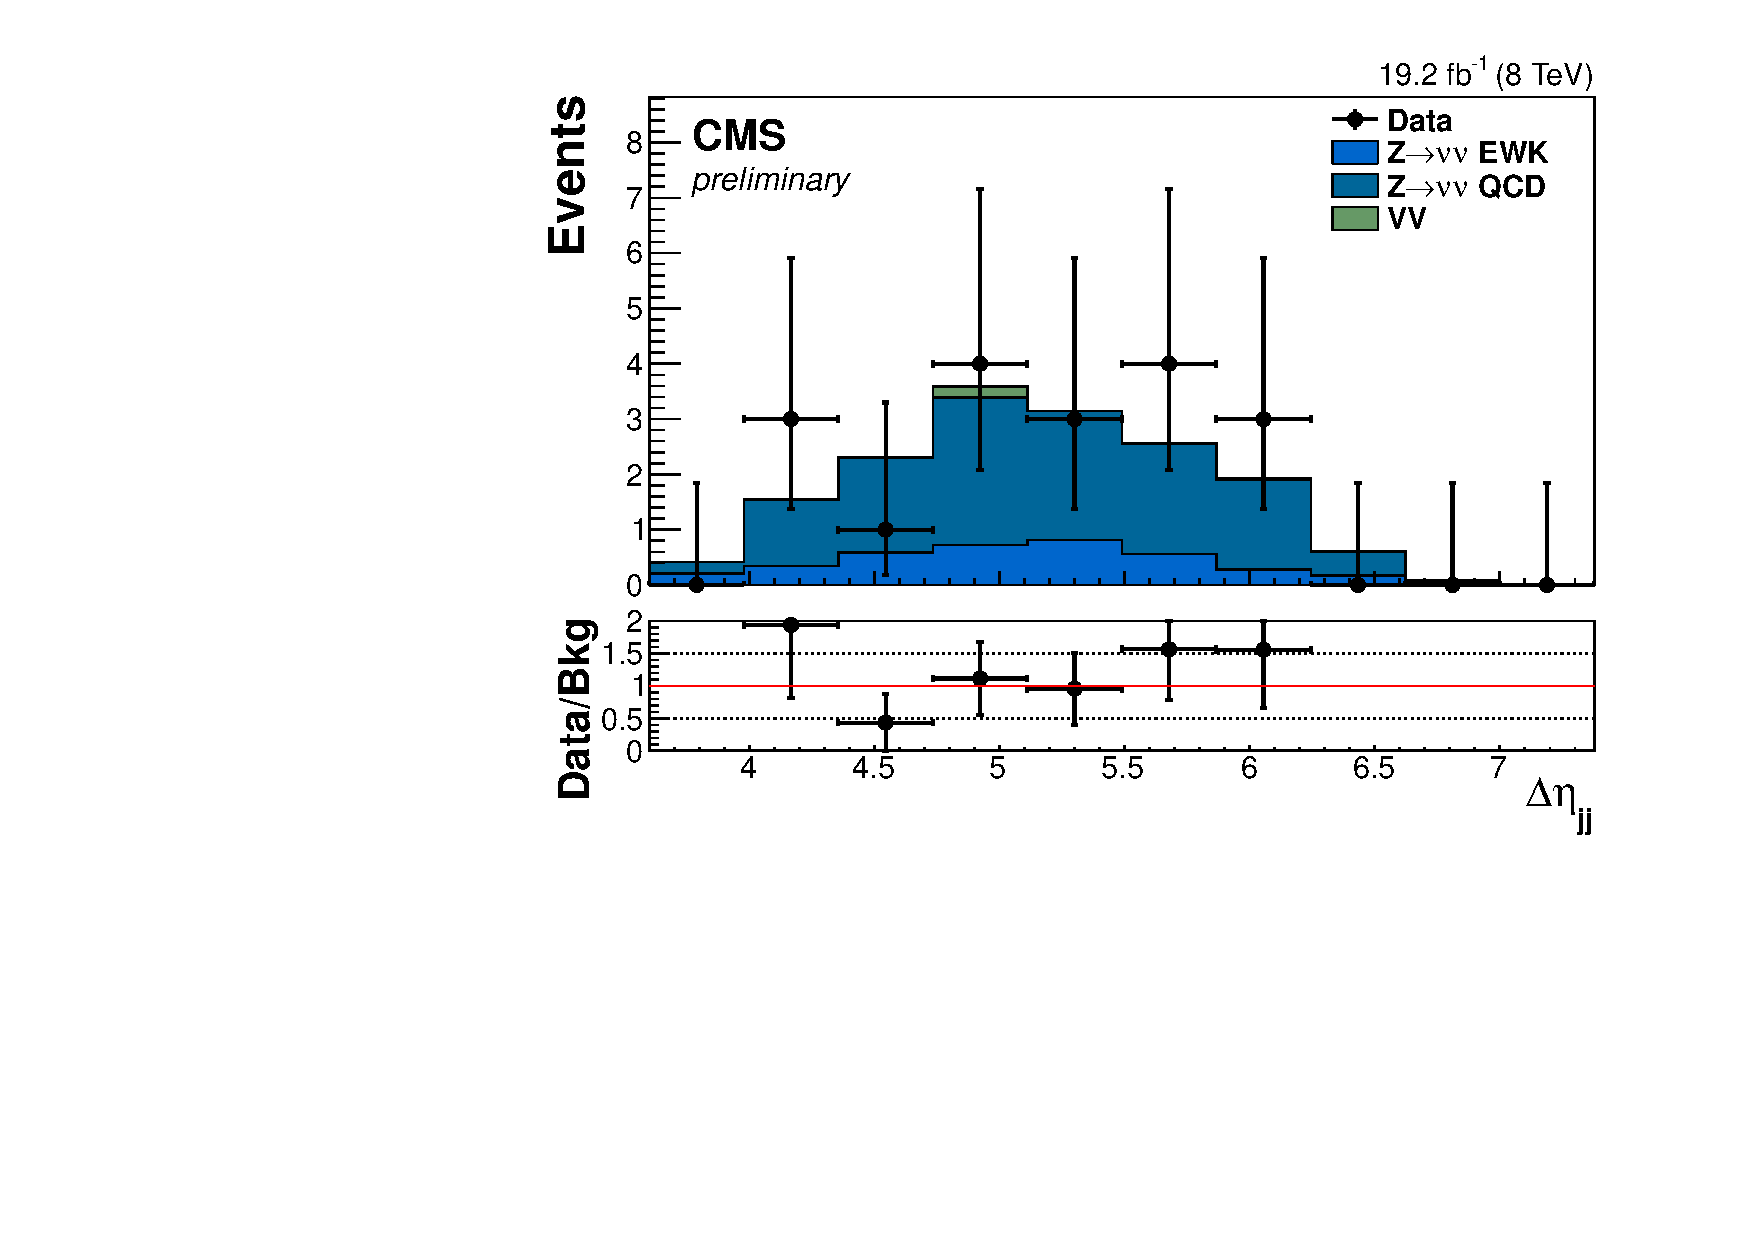
\includegraphics[width=.49\textwidth]{figures/output_sigreg/mumu_dijet_deta.pdf}
%     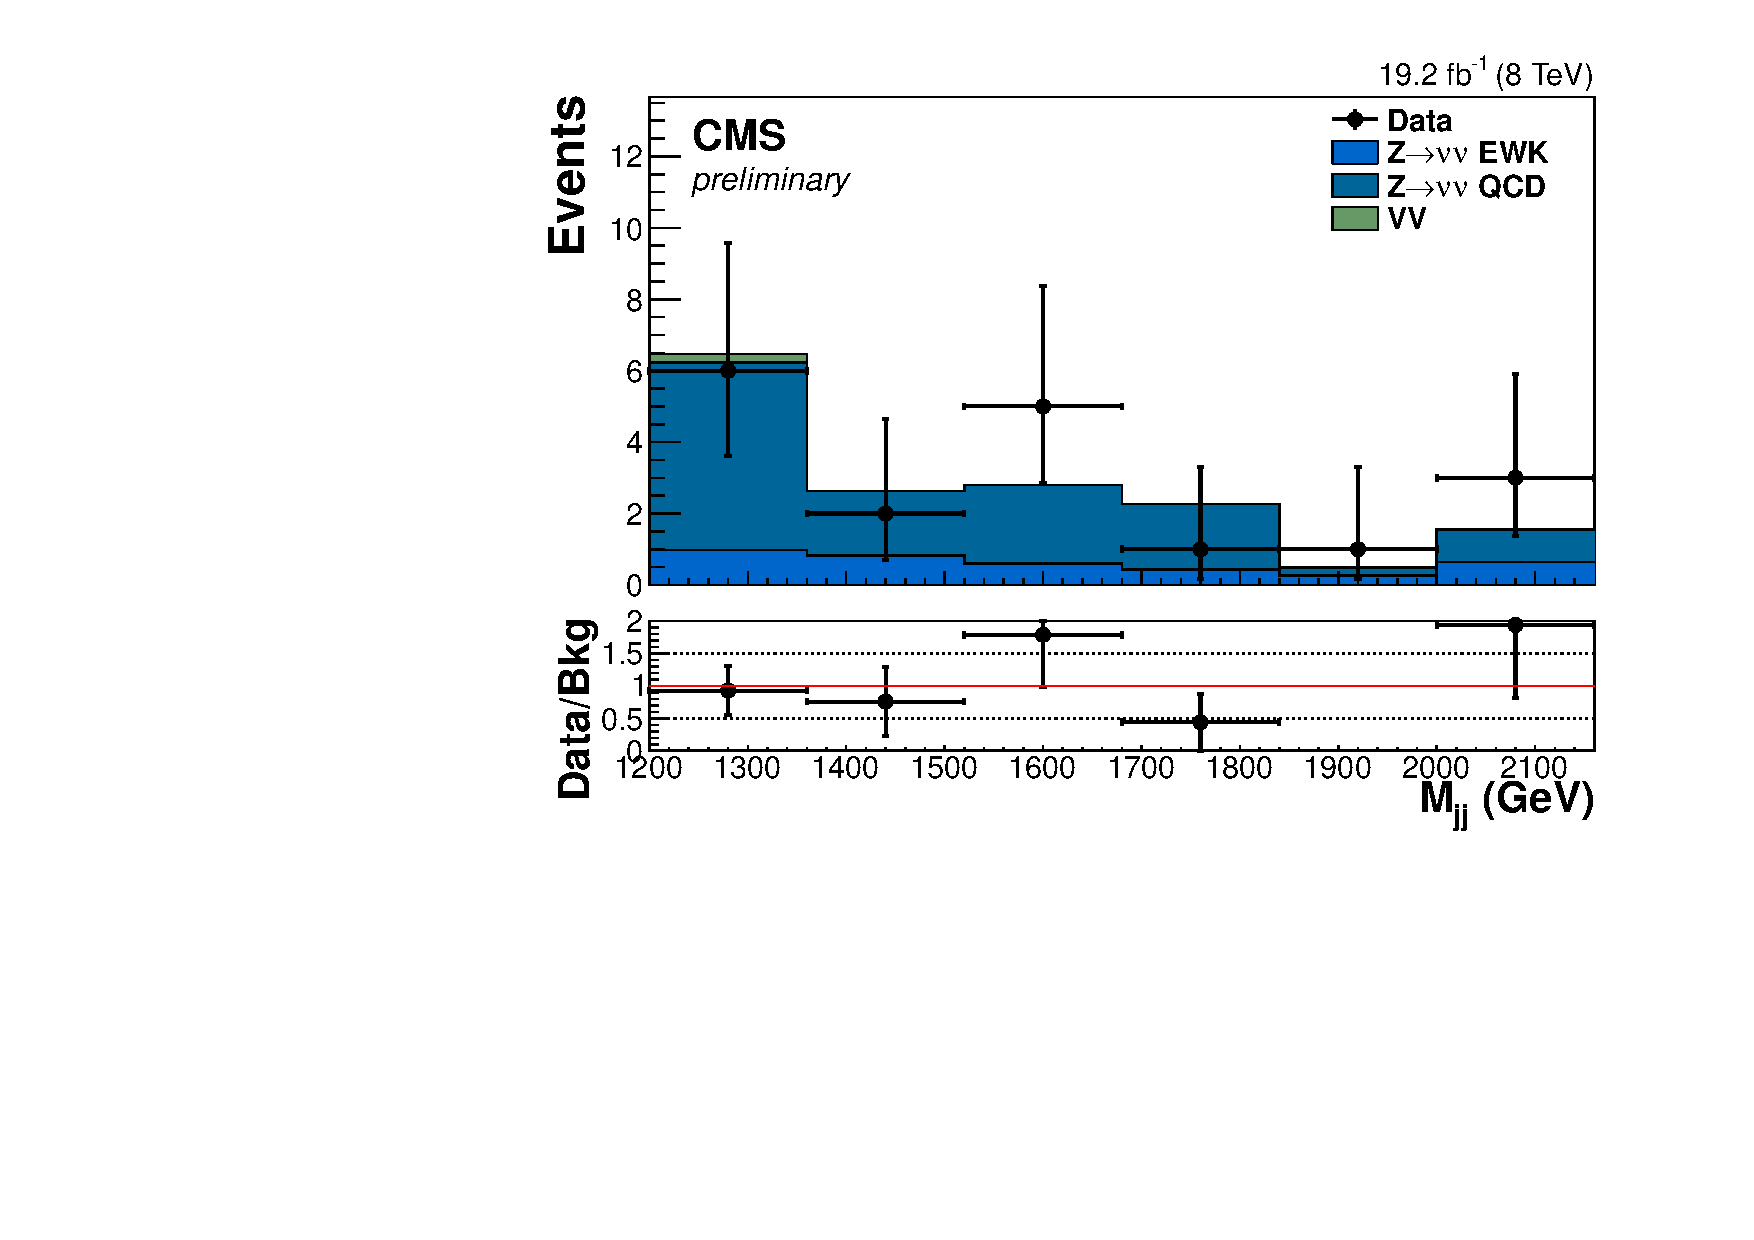
\includegraphics[width=.49\textwidth]{figures/output_sigreg/mumu_dijet_M.pdf}
%     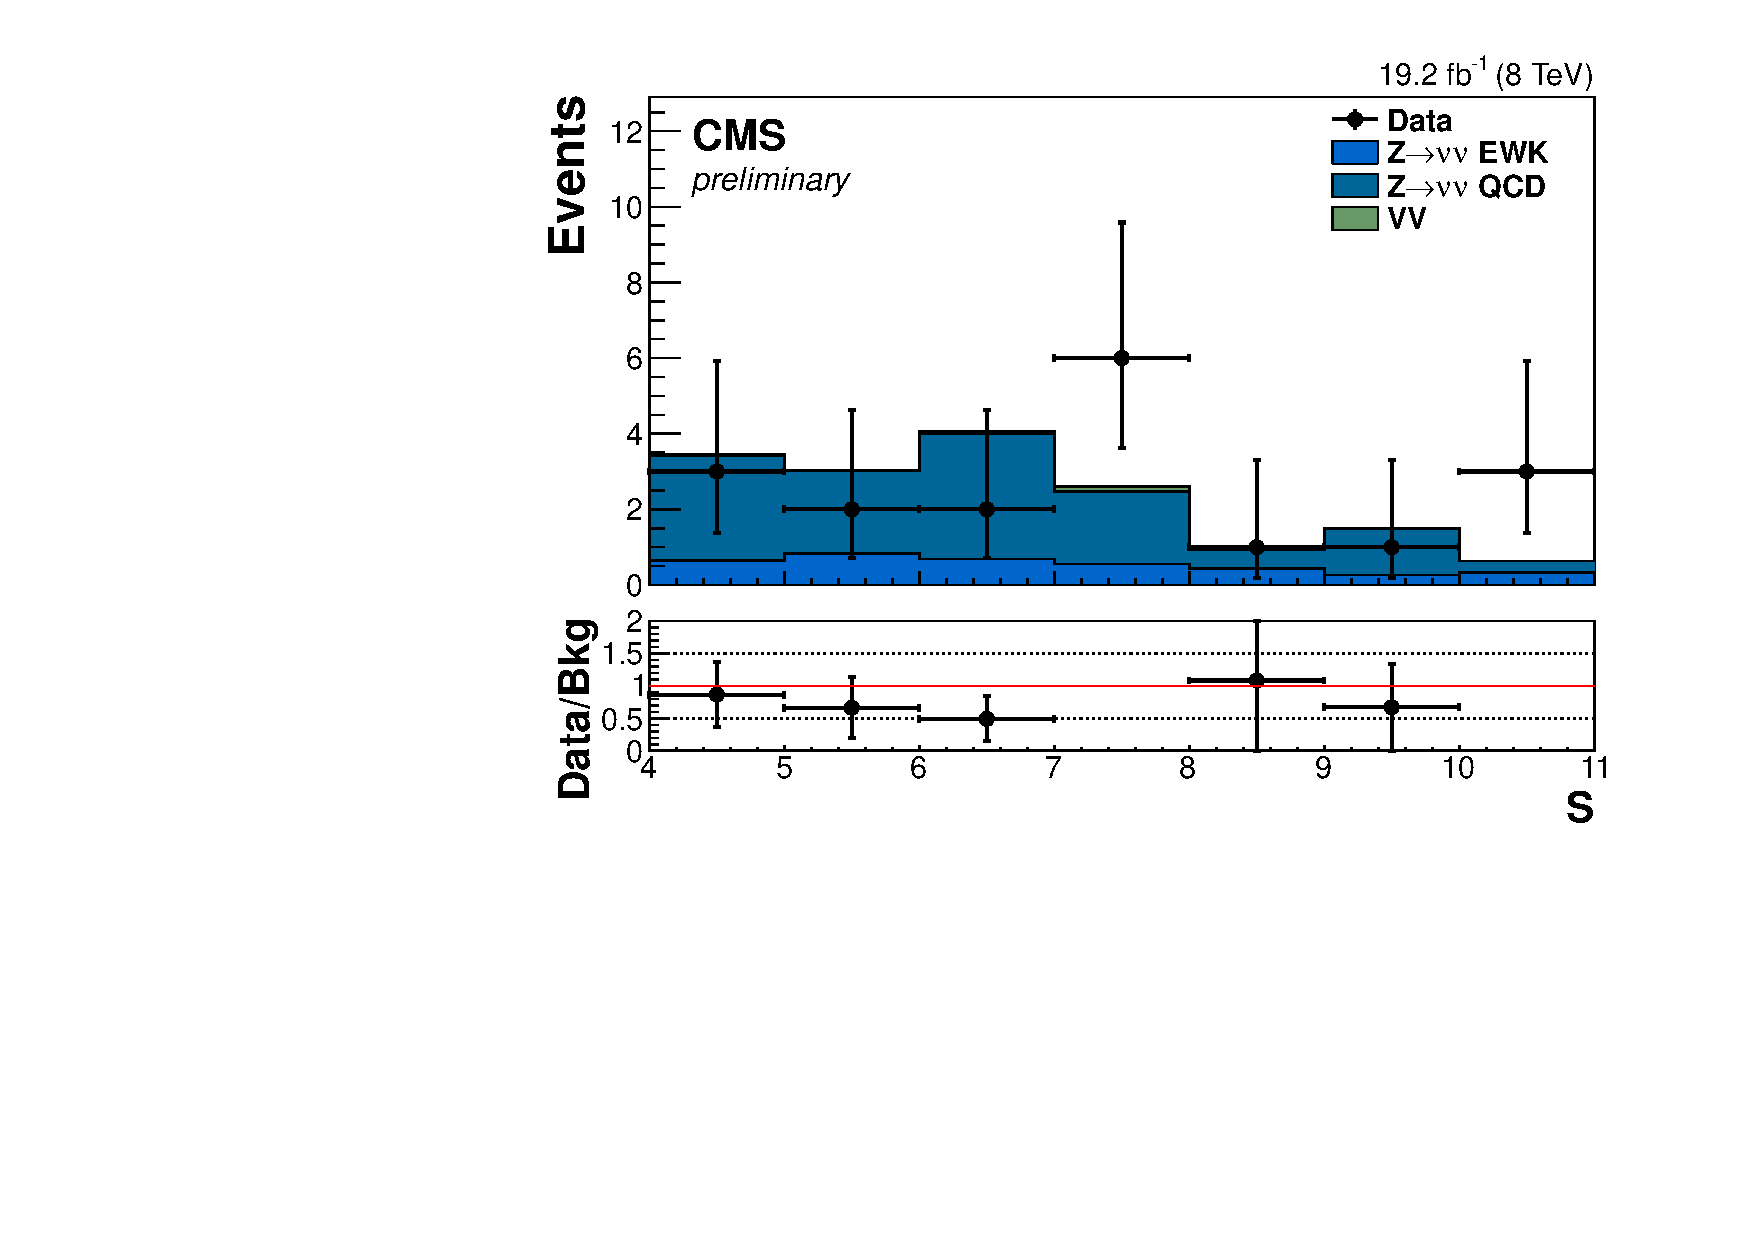
\includegraphics[width=.49\textwidth]{figures/output_sigreg/mumu_metnomu_significance.pdf}
%     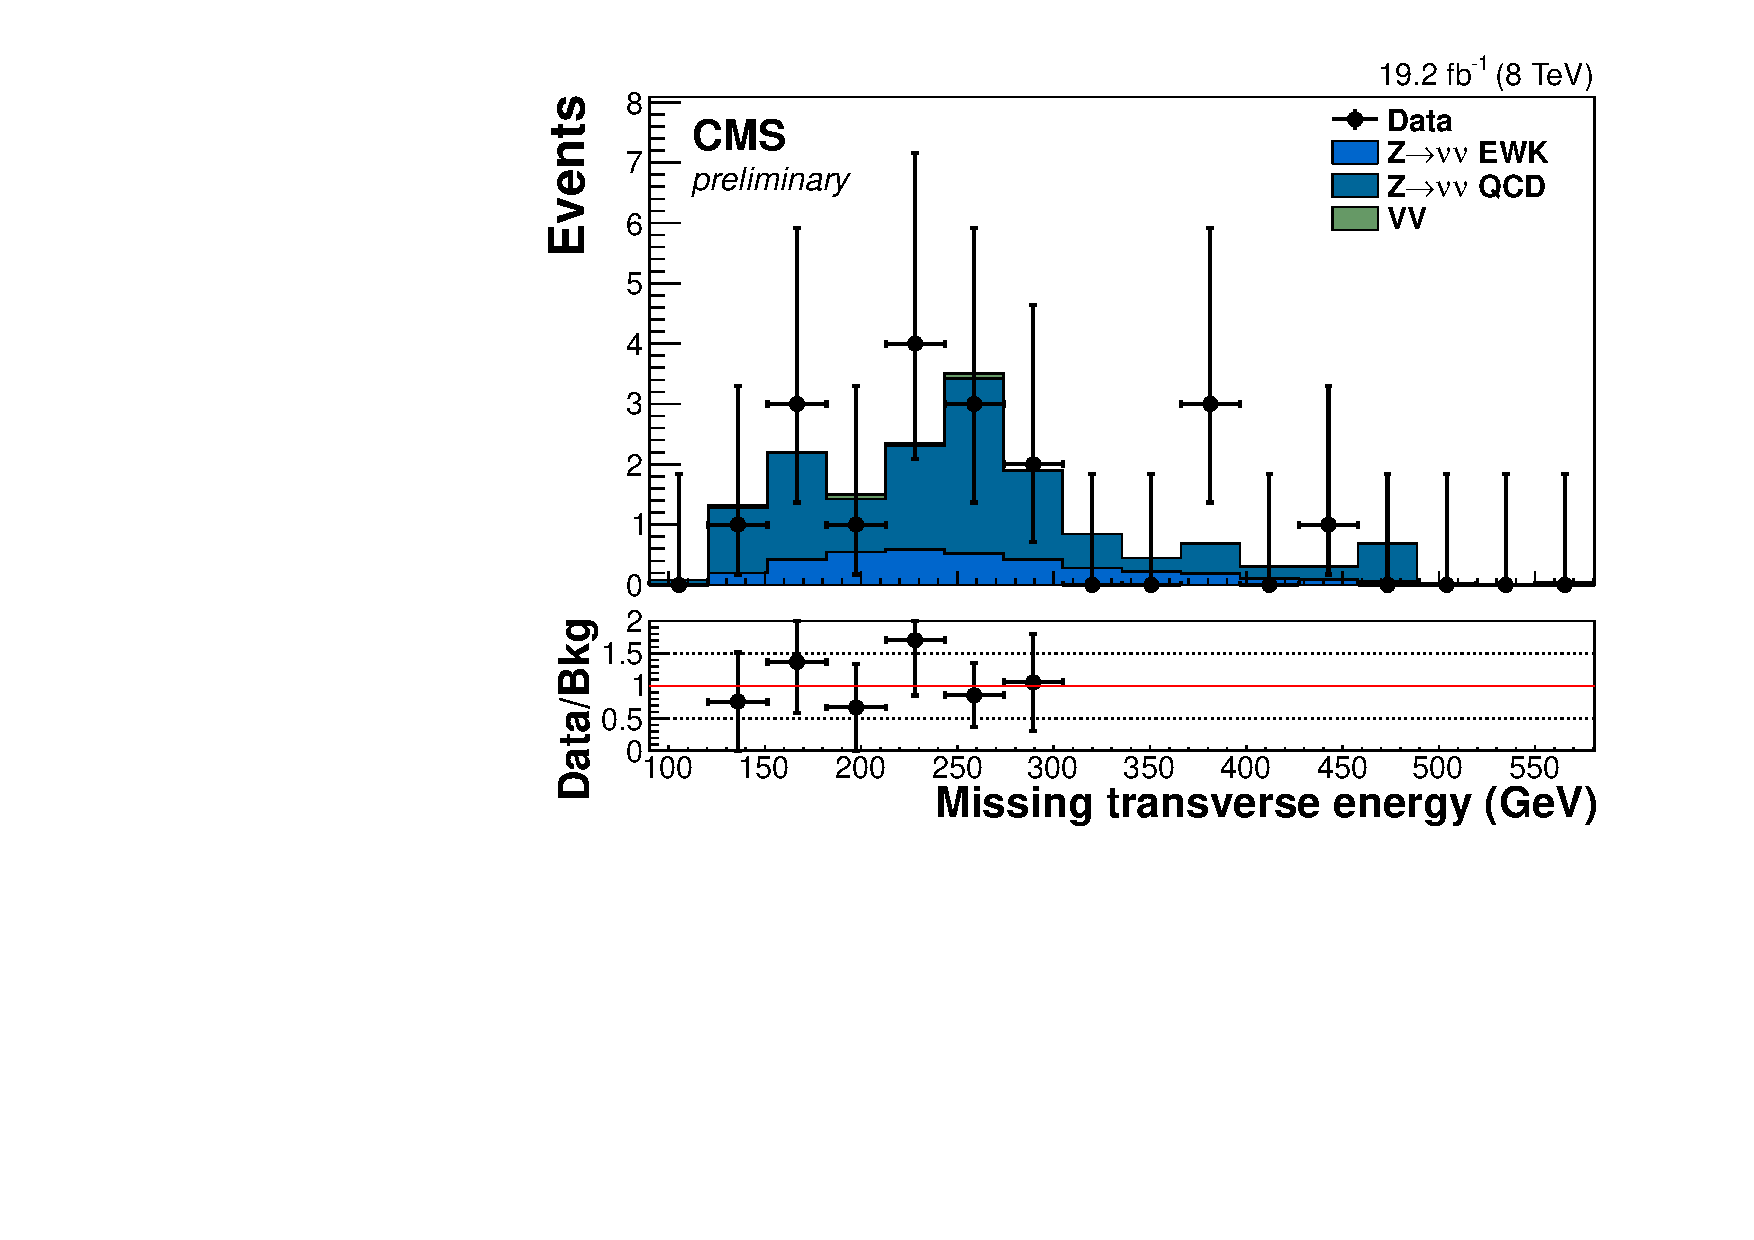
\includegraphics[width=.49\textwidth]{figures/output_sigreg/mumu_metnomuons.pdf}
% 
%     \caption{Top: Pseudorapidity difference between the two VBF tag jets $\Delta\eta_{jj}$ (left), dijet mass $m_{jj}$ (right) bottom: \MET significiance \METsig (left) and \MET (right), in the $Z\rightarrow \mu\mu$ control region. The last bin contains the overflow of the distribution.}
%    \label{fig:mumucontplots}
%   \end{center}
% \end{figure}
% 
% Similarly, in the case of the W background, events in which a lepton
% is explicitly identified are used to compare the MC to data, and
% extract a normalisation factor. This factor is then used to
% normalise the events predicted by the MC in the signal region. The W
% control regions are defined by replacing the signal region's lepton
% veto with a requirement for exactly one lepton (tight electron or
% tight muon) or hadronic tau in order to enrich the sample in W
% events. The number of W events in the signal region is then taken to
% be:
% 
% \begin{align}
%   \begin{split}
%   \label{eq:ddmethod}
%   N_{S}^{W}&=N_{S}^{W\,MC}\frac{N_{C}^{Data}-N_{C}^{bkg}}{N_{C}^{W\,MC}}=N_{S}^{W\,MC}\cdot \rm{SF},
%   \end{split}
% \end{align}
% 
% calculated separately for W decaying to each of e, $\mu$ (with $W\rightarrow\tau\nu\rightarrow e/\mu\nu\nu\nu$ included) and hadronic $\tau$. The number of
% events $N_{C}^{bkg}$ from the backgrounds to the W control regions
% come mainly from the top processes, and are estimated from MC.
% 
% In the W$\rightarrow\tau_{\mathrm{h}}\nu$ control region, almost no
% events pass the \mindphiall selection. The criteria on \mindphiall is
% hence replaced by a criteria on the minimum azimuthal angle separation
% between the \MET and one of the leading two jets, \mindphileading, required
% to be greater than 1. To reject the background from multijet events,
% an additional requirement that the transverse mass of the W be greater
% than 20 GeV is used. By studying the W$\rightarrow\mu\nu$ region
% (which has enough events to observe the full range of the \mindphiall
% distribution), a 20\% systematic uncertainty is added to the
% W$\rightarrow\tau_{\mathrm{h}}\nu$ background estimate to cover the
% small discrepancy in shape of the \mindphiall variable observed
% between data and MC. Distributions of M$_{jj}$, \MET, and \mindphiall
% are shown in Figs.~\ref{fig:wmjjcontplots},\,\ref{fig:wmetcontplots} and \ref{fig:wmindphicontplots}. Good agreement between data
% and MC is observed. The final estimates of the $W\rightarrow l\nu$
% backgrounds, together with the number of events selected in signal and
% control regions, are shown in Table \ref{tab:ZWTopRes}.
% 
% 
% \begin{figure}[h!]
%   \begin{center}
%     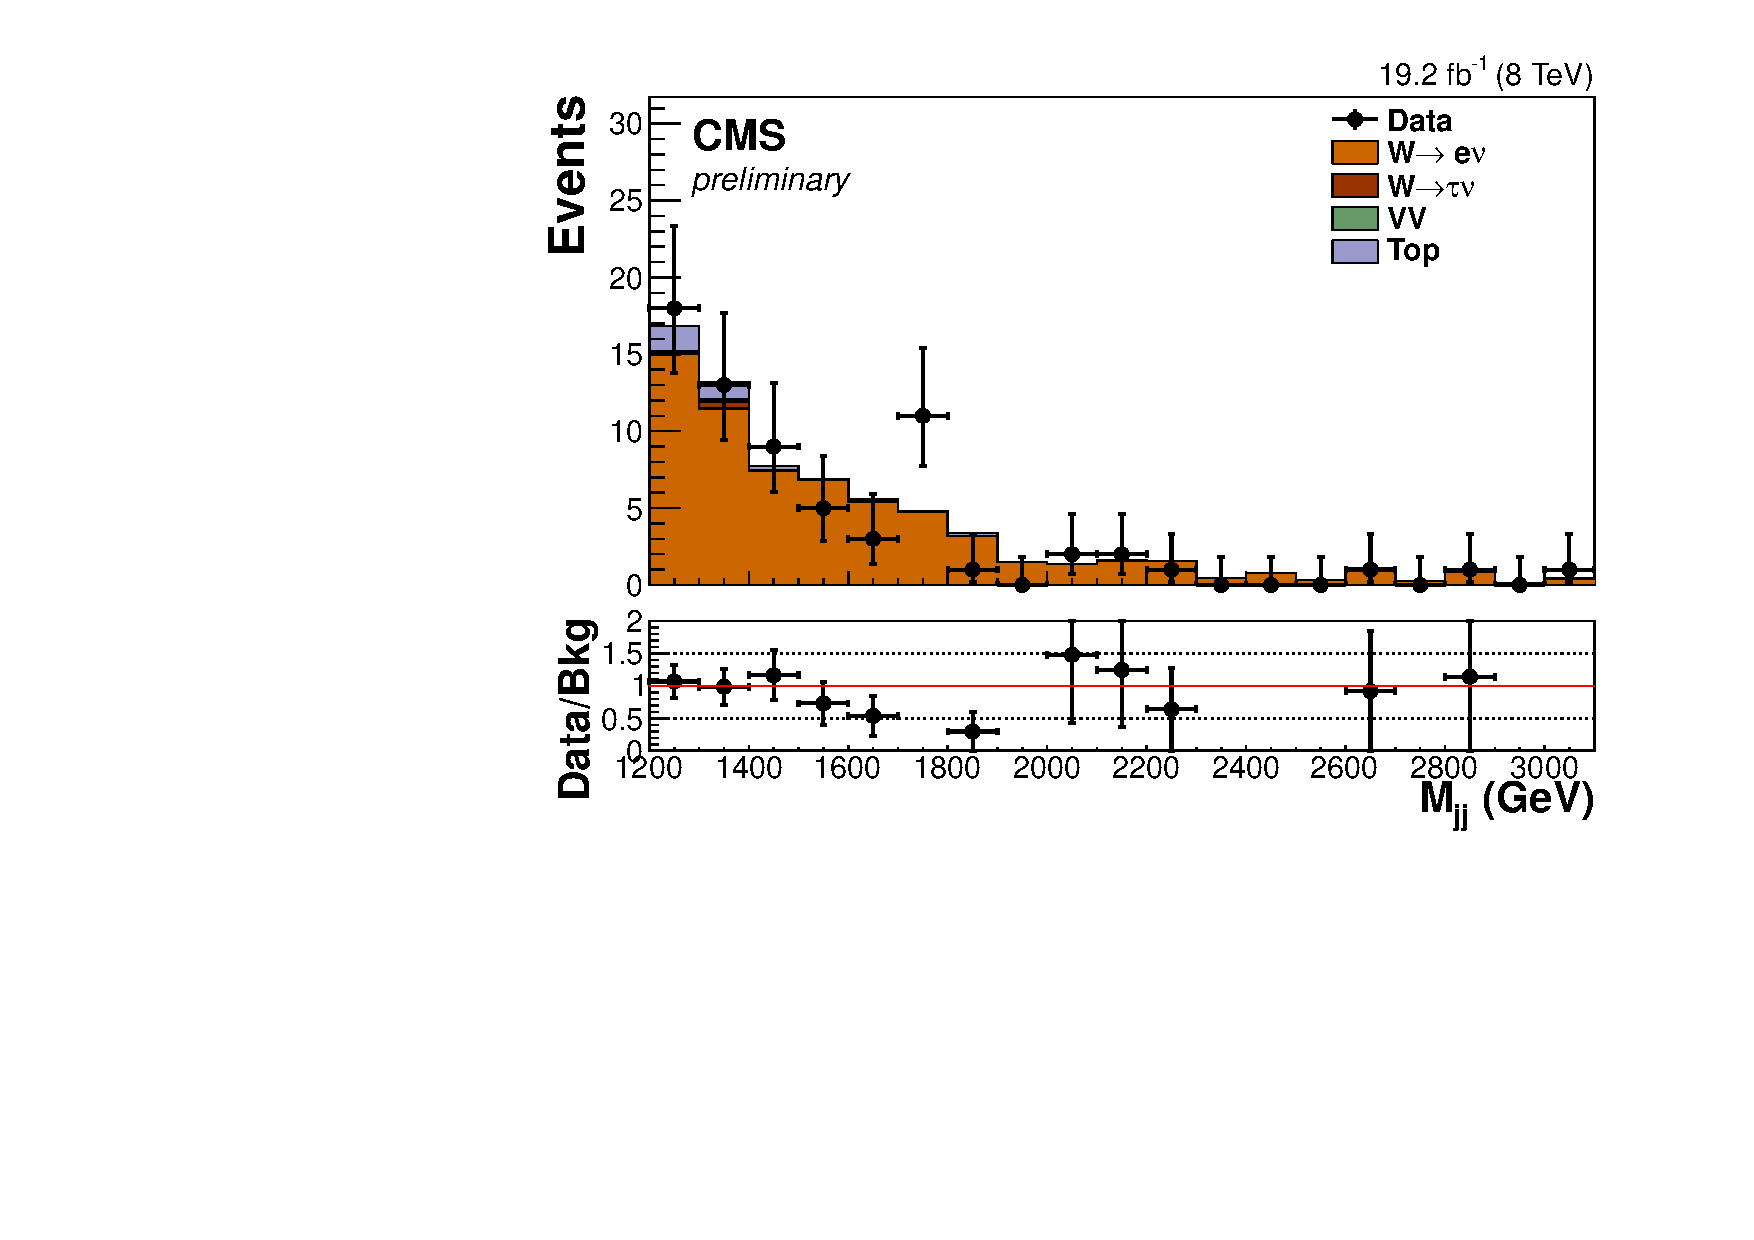
\includegraphics[width=.49\textwidth]{figures/output_sigreg/enu_dijet_M.pdf}
%     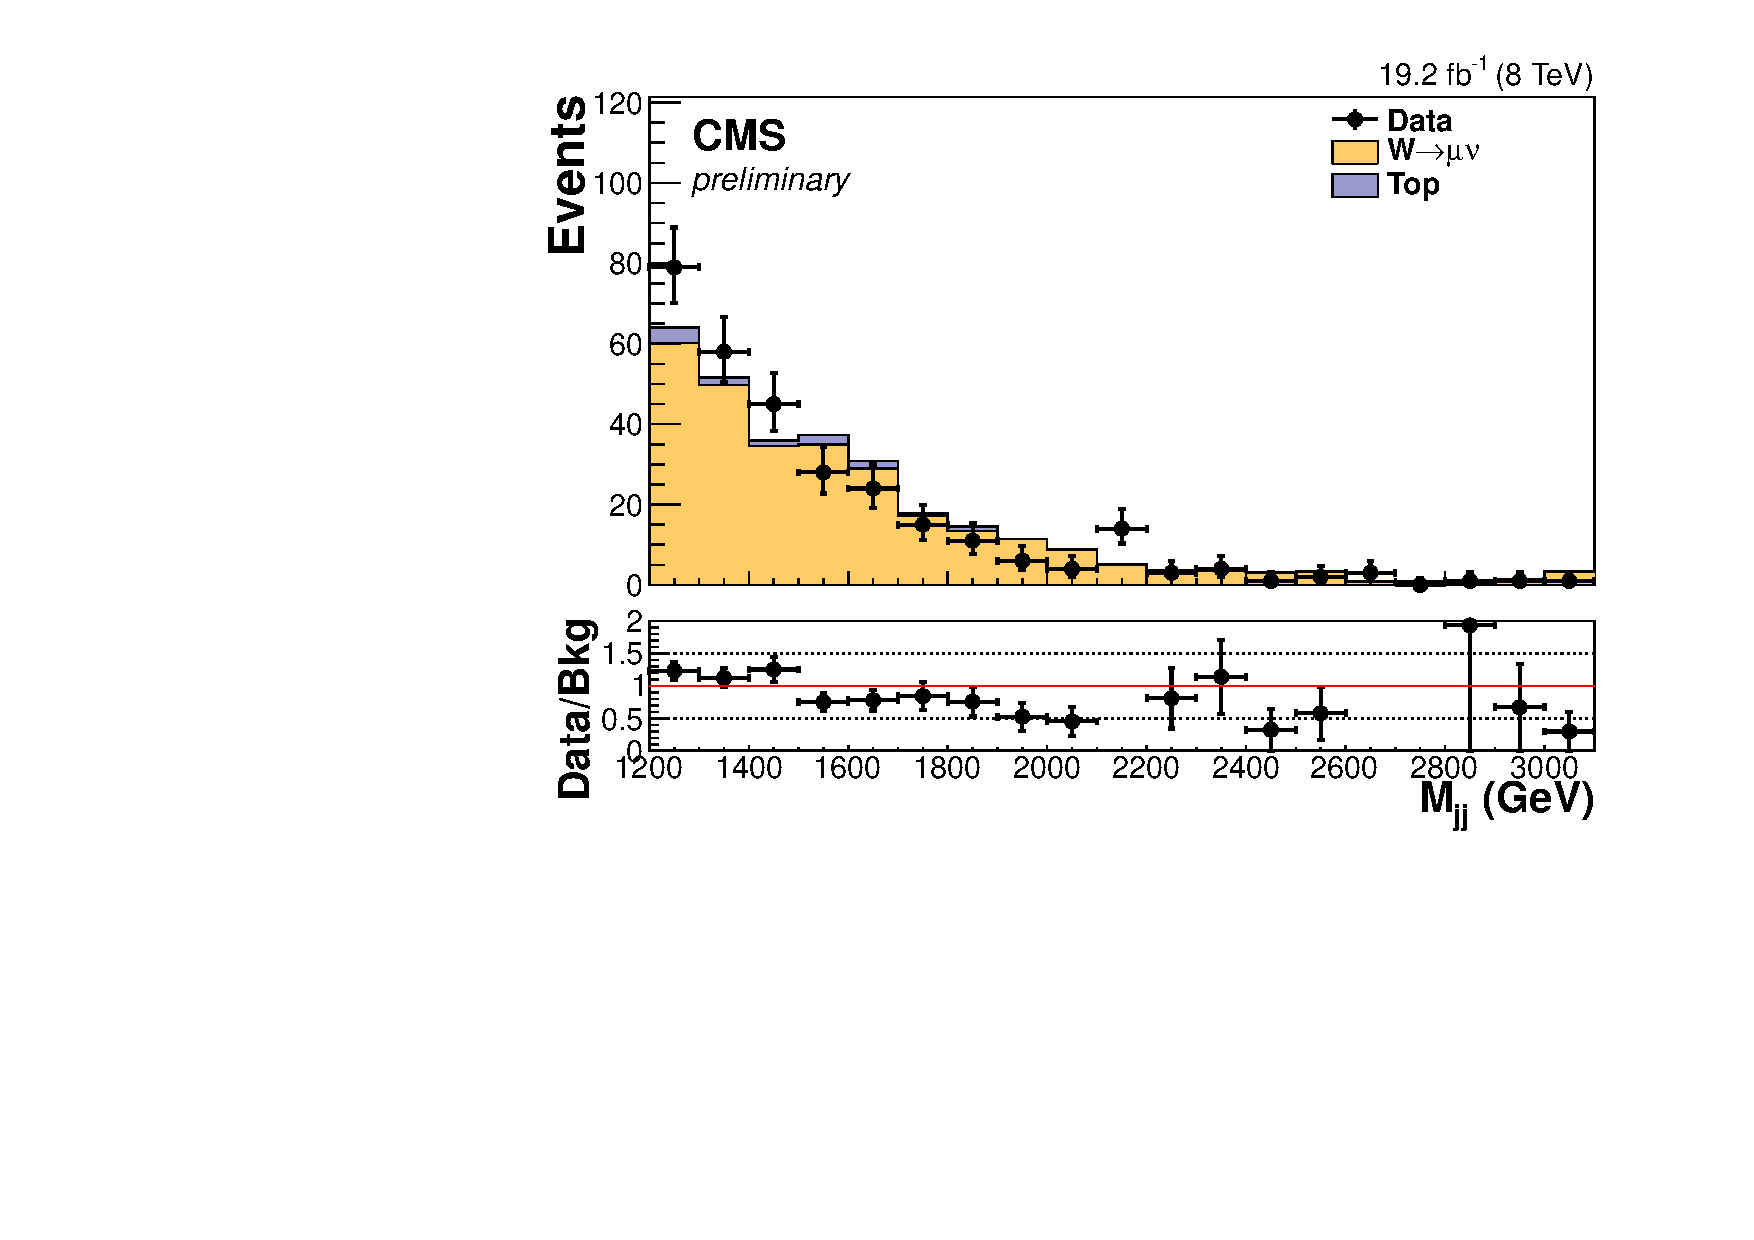
\includegraphics[width=.49\textwidth]{figures/output_sigreg/munu_dijet_M.pdf}
% 
%     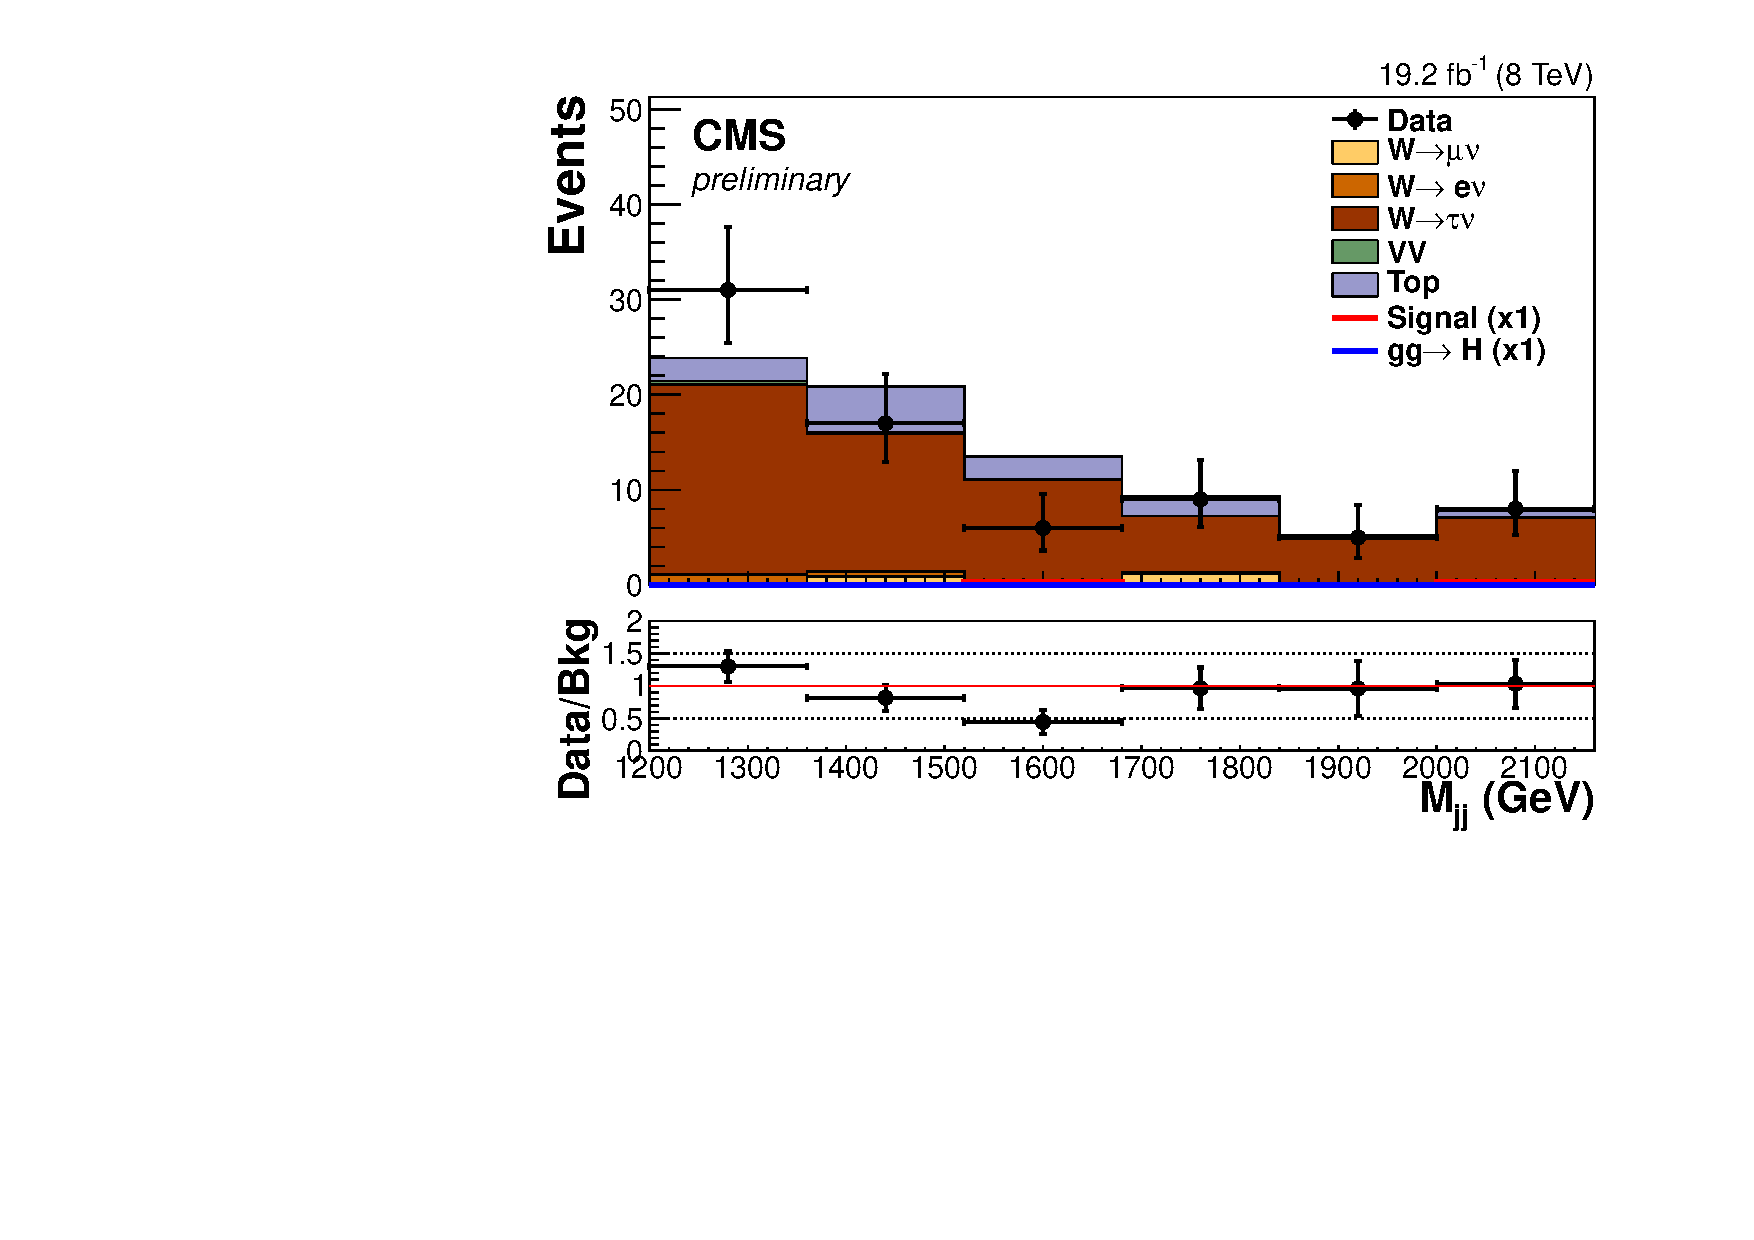
\includegraphics[width=.49\textwidth]{figures/output_sigreg/taunu_dijet_M.pdf}
%     \caption{Dijet mass $m_{jj}$ for the $W\rightarrow e\nu$ (top left), $W\rightarrow\mu\nu$ (top right) and $W\rightarrow\tau\nu$ (bottom) control regions. The last bin represents all those events falling above the range of the histogram.}
%    \label{fig:wmjjcontplots}
%   \end{center}
% \end{figure}
% 
% \begin{figure}[h!]
%   \begin{center}
%     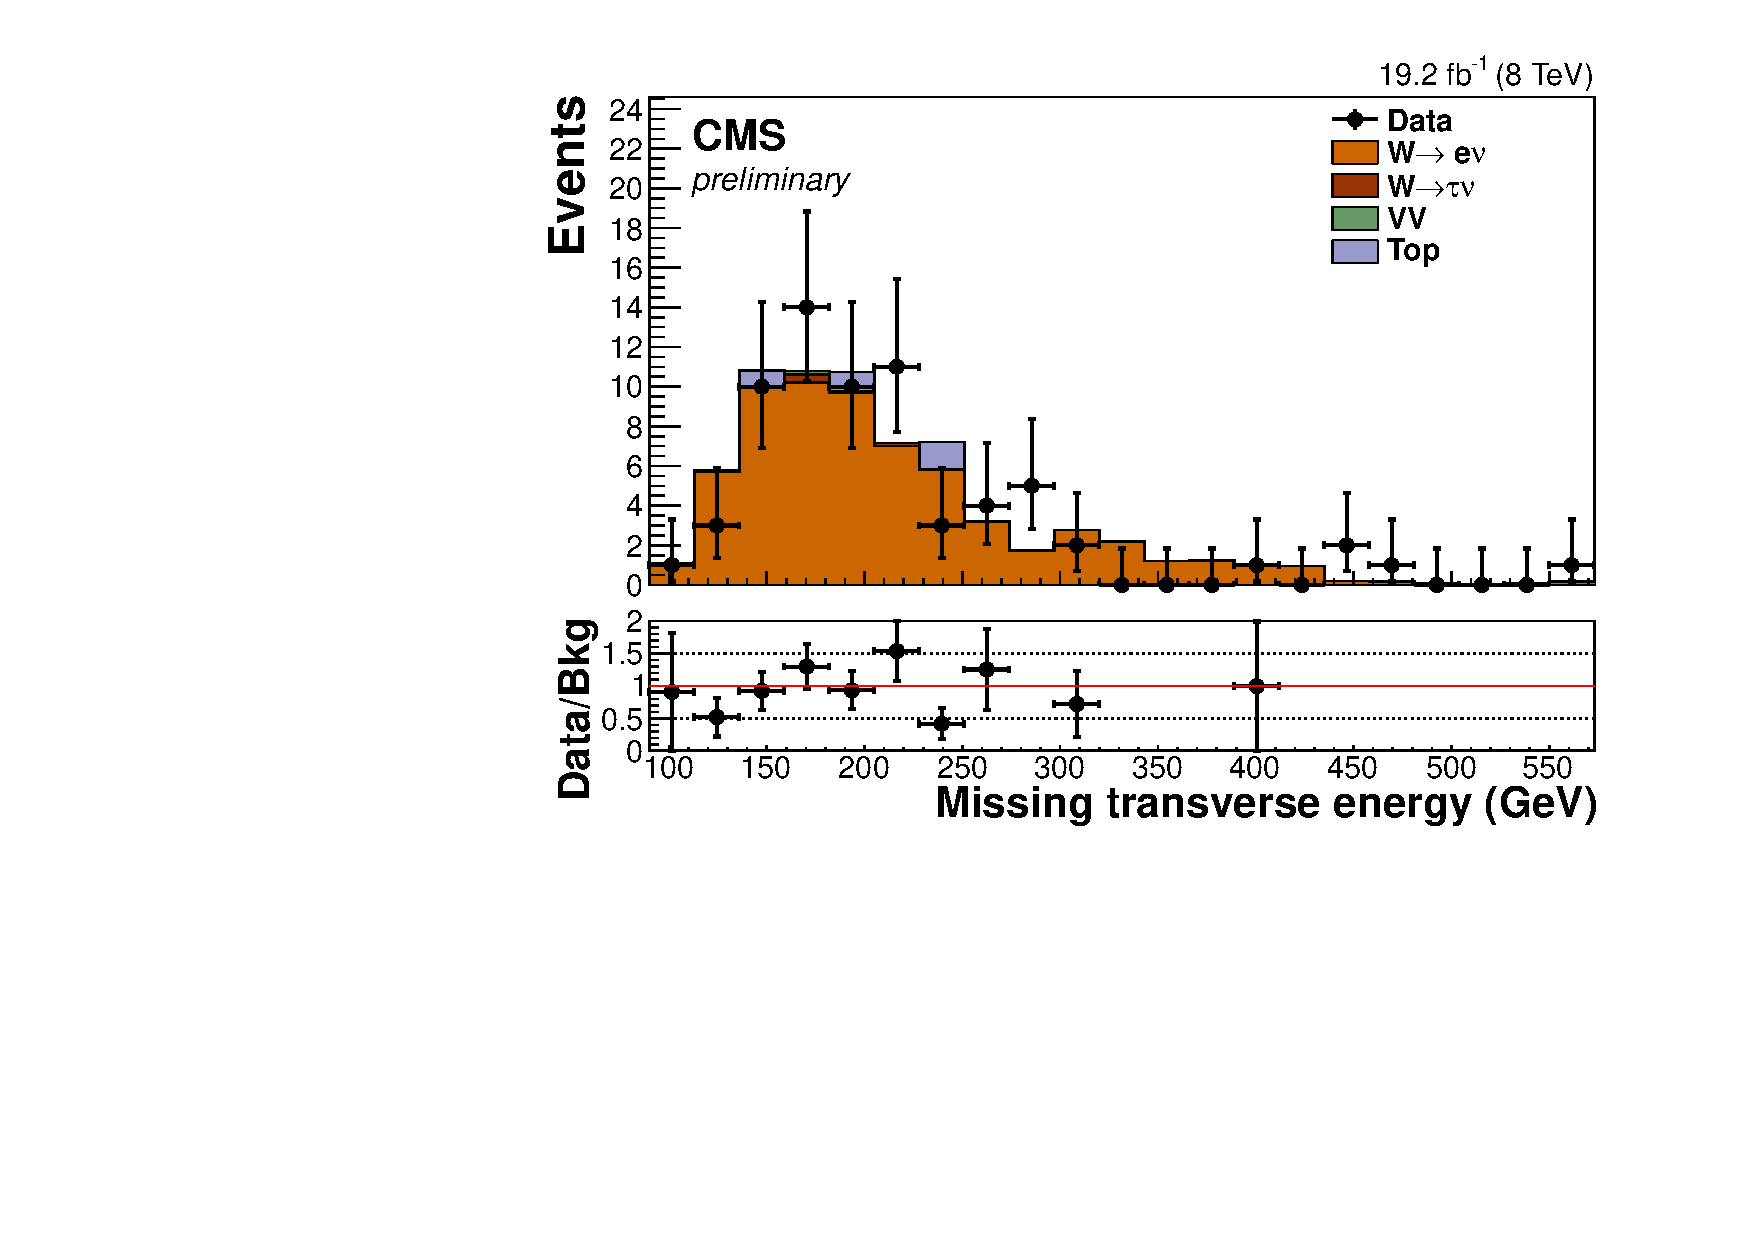
\includegraphics[width=.49\textwidth]{figures/output_sigreg/enu_metnomuons.pdf}
%     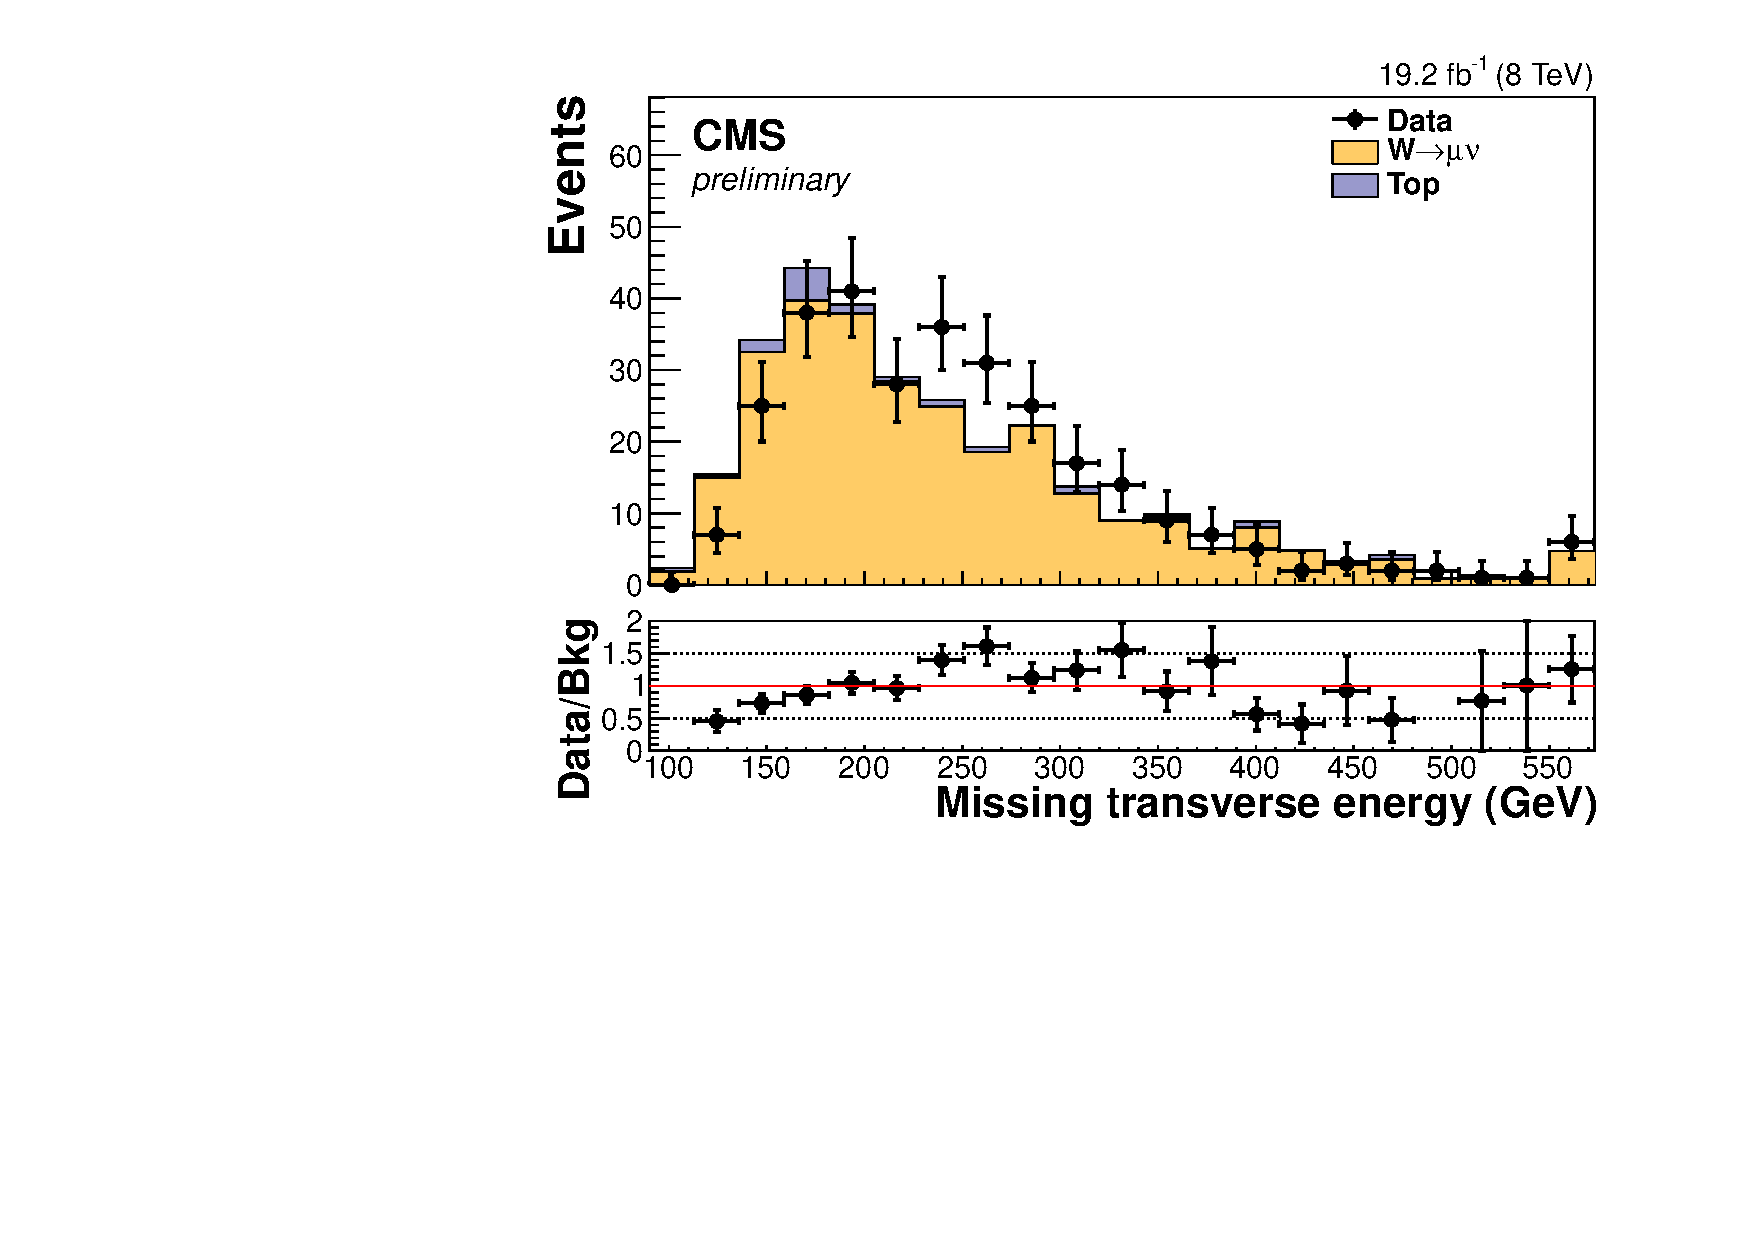
\includegraphics[width=.49\textwidth]{figures/output_sigreg/munu_metnomuons.pdf}
% 
%     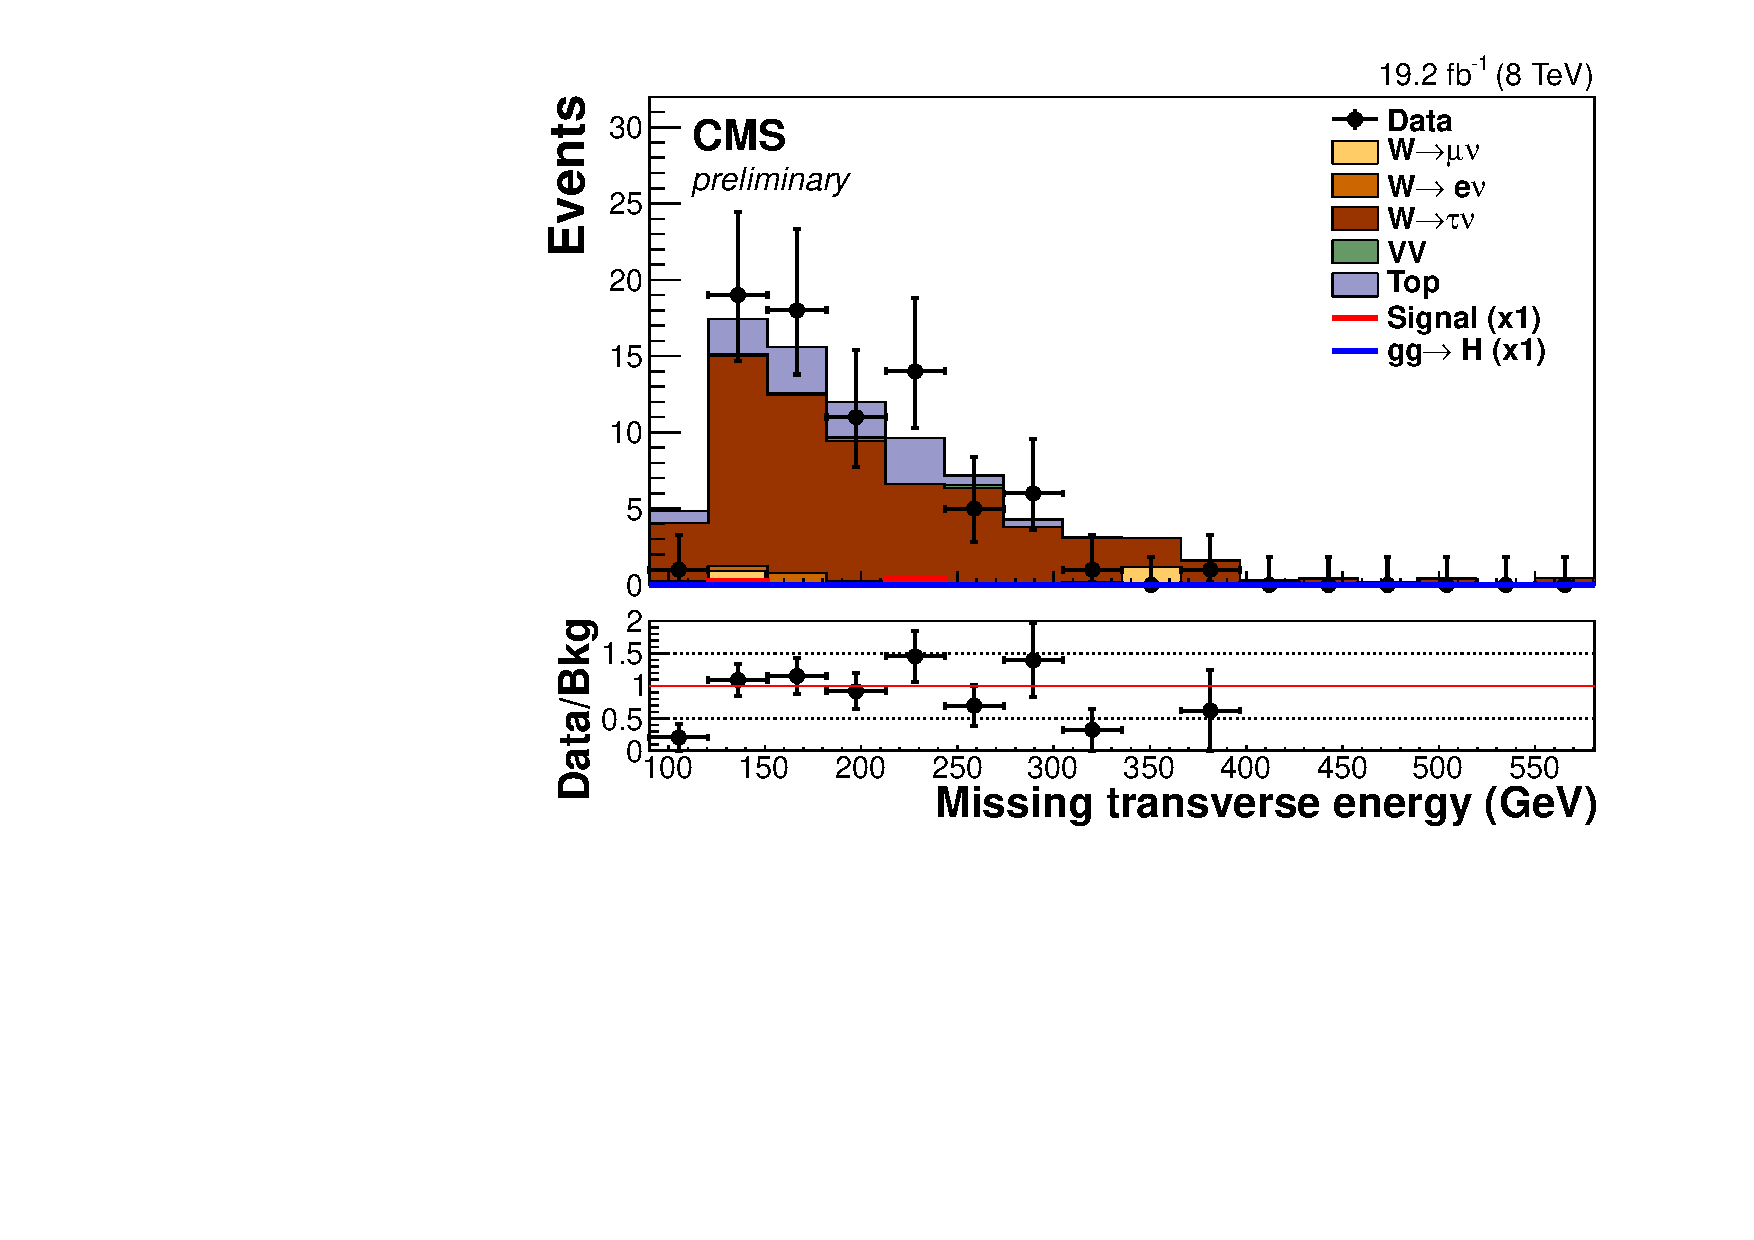
\includegraphics[width=.49\textwidth]{figures/output_sigreg/taunu_metnomuons.pdf}
% 
%     \caption{\MET for the $W\rightarrow e\nu$ (top left), $W\rightarrow\mu\nu$ (top right) and $W\rightarrow\tau\nu$ (bottom) control regions. The last bin represents all those events falling above the range of the histogram.}
%    \label{fig:wmetcontplots}
%   \end{center}
% \end{figure}
% 
% \begin{figure}[h!]
%   \begin{center}
%     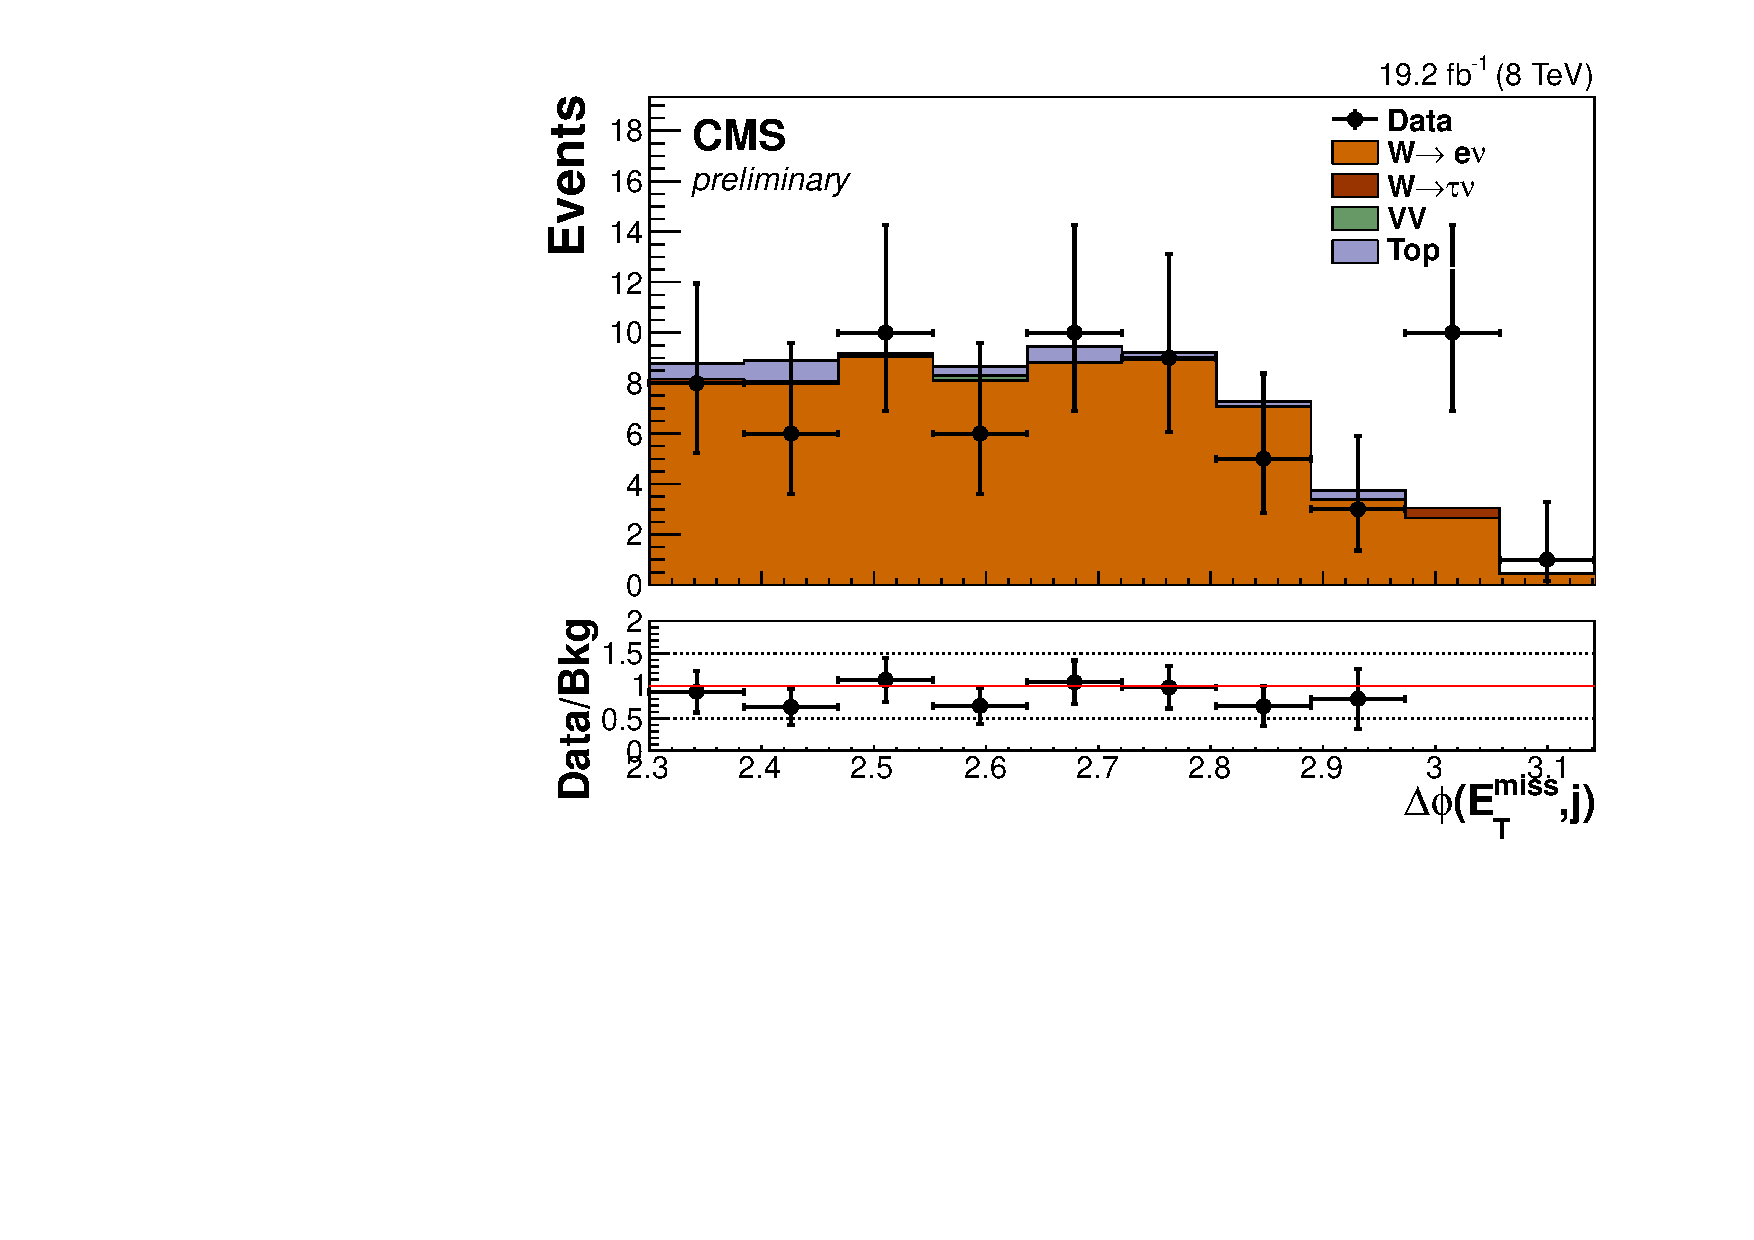
\includegraphics[width=.49\textwidth]{figures/output_sigreg/enu_alljetsmetnomu_mindphi.pdf}
%     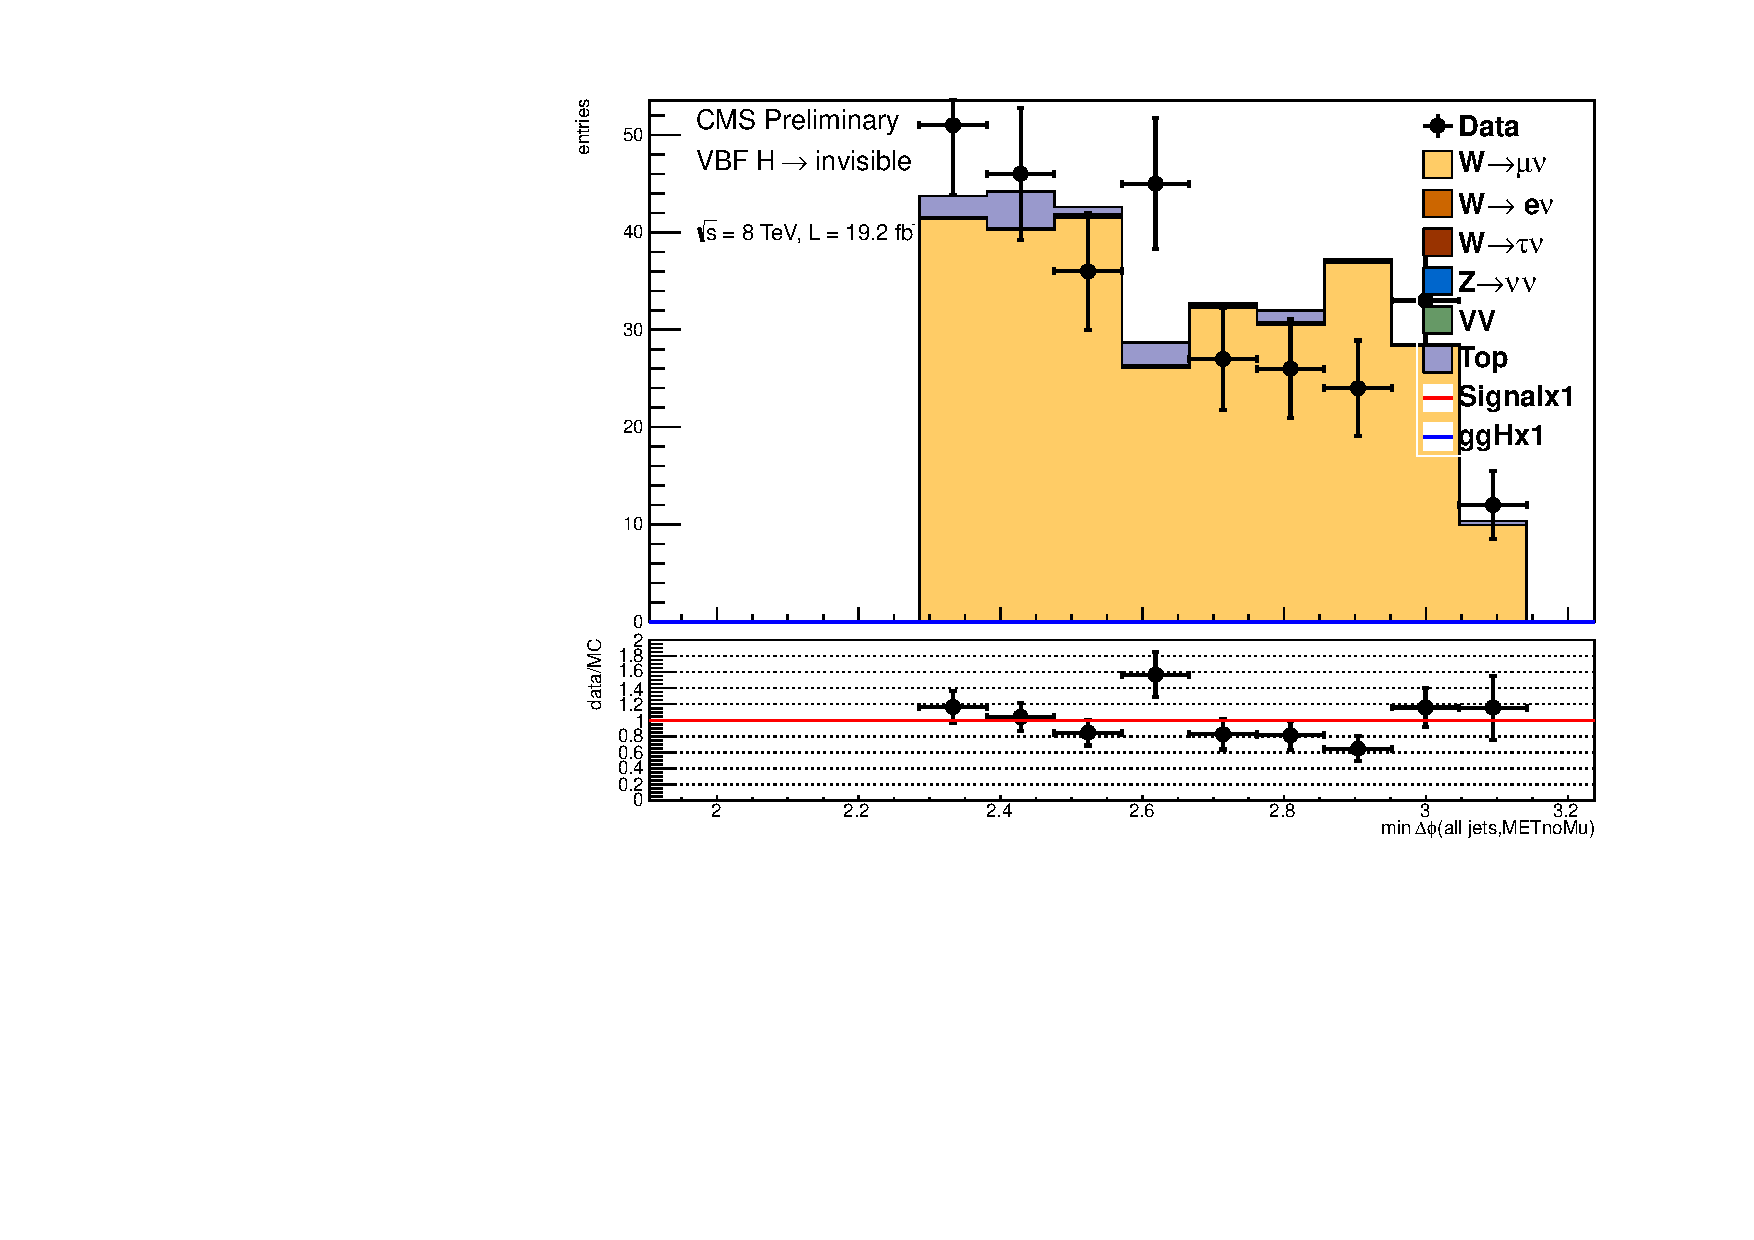
\includegraphics[width=.49\textwidth]{figures/output_sigreg/munu_alljetsmetnomu_mindphi.pdf}
% 
%     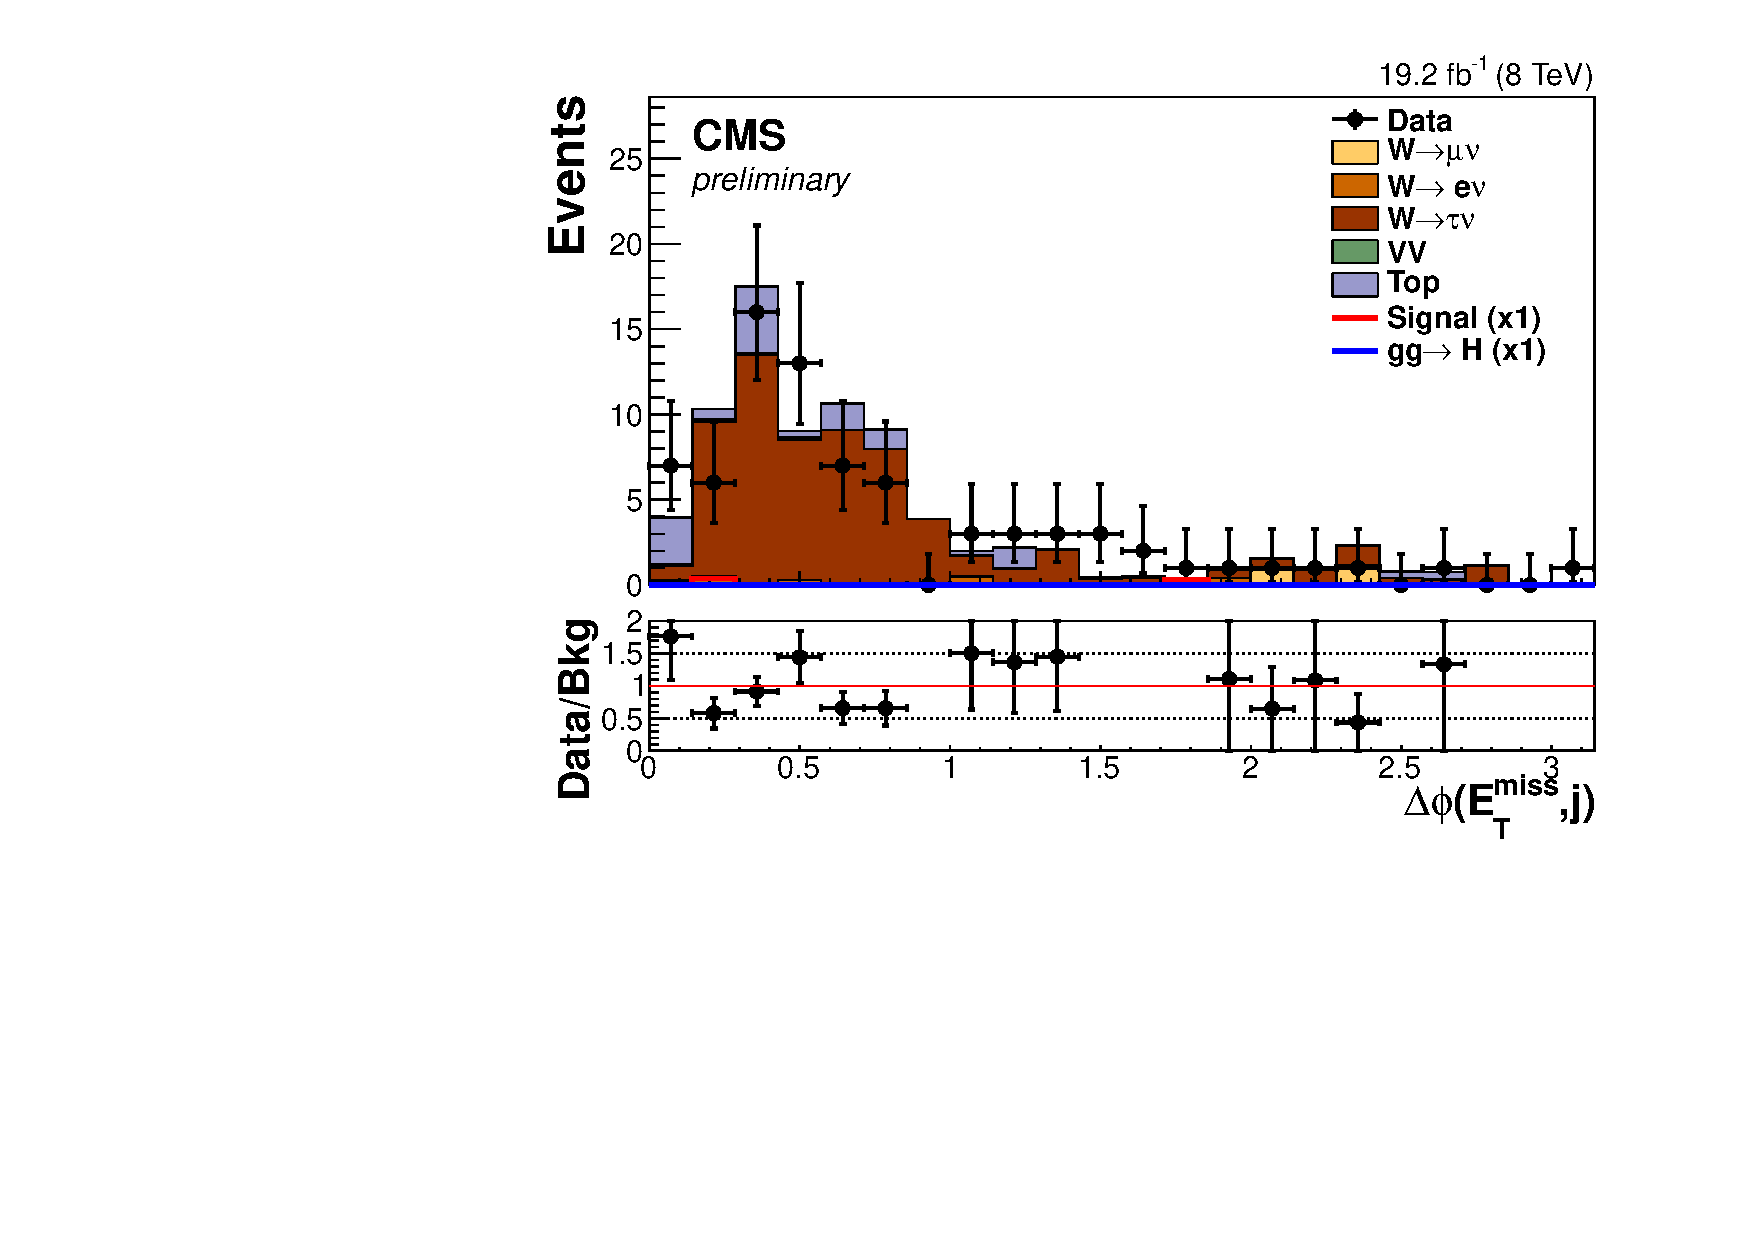
\includegraphics[width=.49\textwidth]{figures/output_sigreg/taunu_alljetsmetnomu_mindphi.pdf}
%     \caption{Minimum azimuthal angle separation between any jet with $p_{T}>30$ GeV and the \MET \mindphiall for the $W\rightarrow e\nu$ (top left), $W\rightarrow\mu\nu$ (top right) and $W\rightarrow\tau\nu$ (bottom) control regions.}
%    \label{fig:wmindphicontplots}
%   \end{center}
% \end{figure}
% 
% 
% \begin{table}[h!]
% \begin{center}
%   \topcaption{\label{tab:ZWTopRes} Summary of the W background estimates.
%     The quoted uncertainties are of statistical origin. Systematic uncertainties are shown, as well, for
%     SF and $N_S$. Systematic uncertainties are
%     described in Section~\ref{sec:syst}. The systematic
%     uncertainty given for SF contains only the MC statistics, whereas for $N_{S}$ it represents the full systematic as described in section \ref{sec:syst}.}
% 
% \begin{tabular}{|l|c|c|c|}
% \hline
%  & W$\rightarrow$e$\nu$ & W$\rightarrow\mu\nu$ & W$\rightarrow\tau\nu$ \\
%  \hline
% $N_{C}^{data}$ & $68\pm 8.2$& $300\pm 17.3$ & $76\pm 8.7$\\
% $N_{C}^{bkg}$   &$3.5\pm 1.2$ & $14.8\pm 2.5$ & $13.3\pm 2.8$ \\
% $N_{C}^{MC}$ &  $128.0\pm 8.0$ & $399.9\pm 14.9$ & $80.8\pm 6.4$   \\
% $N_{S}^{MC}$ & $114.9\pm8.9$ & $143.7\pm10.2$ & $121.9\pm8.7$  \\
%  \hline
%  SF & $0.50\pm0.06\pm0.03$ & $0.71\pm0.04\pm0.03$ & $0.78\pm0.11\pm0.07$ \\
%  \hline
% $N_{S}$ & $57.9\pm7.4\pm7.7$ & $102.5\pm6.2\pm11.7$ & $94.6\pm13.1\pm23.8$ \\
%  \hline
% \end{tabular}
% \end{center}
% \end{table}
% 
% The data-to-simulation scale factors shown in Table~\ref{tab:ZWTopRes} vary from
% 0.5 to 0.8. This difference is caused by a mismodelling of the distribution of the 
% dijet mass and \mindphiall variables; tighter requirements on these variables lead to decreasing
% scale factors.
% 
% Two top control regions have also been investigated. One (region 1) is
% driven by the selection of two leptons, either of different flavour (e$\mu$), or
% of the same flavour (ee or $\mu\mu$) with a veto on the Z mass region.
% This region is found to be composed almost entirely of \ttbar
% events. The other (region 2) is based on the selection of one lepton (e
% or $\mu$), and the requirement that one of the two leading jets is identified as a jet from a b quark
% (using the Combined Secondary Vertex algorithm ~\cite{Chatrchyan:2012jua}). This region is found to be composed of 10\%
% single top, 50\% \ttbar and 40\% W+jets. The number of events expected from simulation is found to be in good agreement with the
% observed number of events in both control regions. The data-to-simulation scale factors obtained are
% $1.21\pm 0.19$ (data stat.)$ \pm 0.16 $(syst.) from 21 events observed in region 1 and
% $0.88\pm 0.07$ (data stat.)$ \pm 0.08$ (syst.) from 429 events observed in region 2.
% The systematic uncertainty in these scale factors is dominated by the limited statistics in the simulation.
% Based on these results we assign a 20\% systematic uncertainty to the nominal prediction for the top quark contribution
% in the signal region.
% 
% %The grey shaded band in the signal region figure is the total
% %systematic and statistical uncertainty on the total background
% %estimation. It should be noted that the QCD contribution, estimated at
% %17 events across the distribution, is not shown. 
% %All plots have the W, Z and top backgrounds normalised to the
% %date in their respective control regions
% 
% For the QCD background, a data-based method using events with non-isolated \MET is employed. Three
% regions are defined: (i) a region denoted as "inverted" that 
% gives a description of the QCD shape; (ii) a region denoted as "3-jet"
% where a cross-check of how well the QCD shape
% describes the data is performed; and (iii) a region denoted as "sideband" from which
% a normalisation of the QCD shape to be applied in
% the signal region is extracted.
% 
% The inverted region is selected by changing the requirement on
% \mindphiall to \mindphiall$<$1.0, and requiring \mindphileading $>$ 2.3, thus providing a region where the leading two jets are signal like, but the \MET is not isolated.
%  The distribution of \METsig is shown after this
% inverted selection in Fig.~\ref{fig:invqcd} (left). About 20\% of the
% events are expected to come from W, Z and top processes. The QCD
% shape is defined as the shape of the data in this region after subtracting the MC predictions for the non QCD processes which are normalised by the SF determined from the corresponding control regions selected in the same conditions as the inverted region. Good
% agreement is found between the data and the shape predicted by the VBF-enriched QCD MC simulation in this region as shown in Fig.~\ref{fig:invqcd}
% (left).
% 
% To ensure that the QCD shape is adequate to describe the isolated \MET the 3-jet
% QCD-dominated control region is defined by requiring \mindphiall$>1$, \METsig$>3$ and at least three jets with p$_{T}>30$\,GeV.
% From simulation we expect a negligible contribution from signal after requiring a third jet in the event. The expected number of QCD events
% in the 3-jet region, n$_{QCD}^{3j}$, is then taken as the
% background-subtracted data, with the W and Z expectations being
% normalised to their respective leptonic control regions.  We then compare the QCD shape, taken from the inverted region with \mindphileading$>1.0$ and normalised to n$_{QCD}^{3j}$, with the data in this region. The distribution of \METsig is shown in this
% QCD-enriched selection in Fig.~\ref{fig:invqcd} (right). The discrepancy between data and prediction in this QCD-dominated 3-jet region is found to be less than 20\%. However, because most of the events passing
% the final selection have only two jets, this control region can not be
% used in the final QCD estimate.
% 
% \begin{figure}[h!]
%   \begin{center}
%     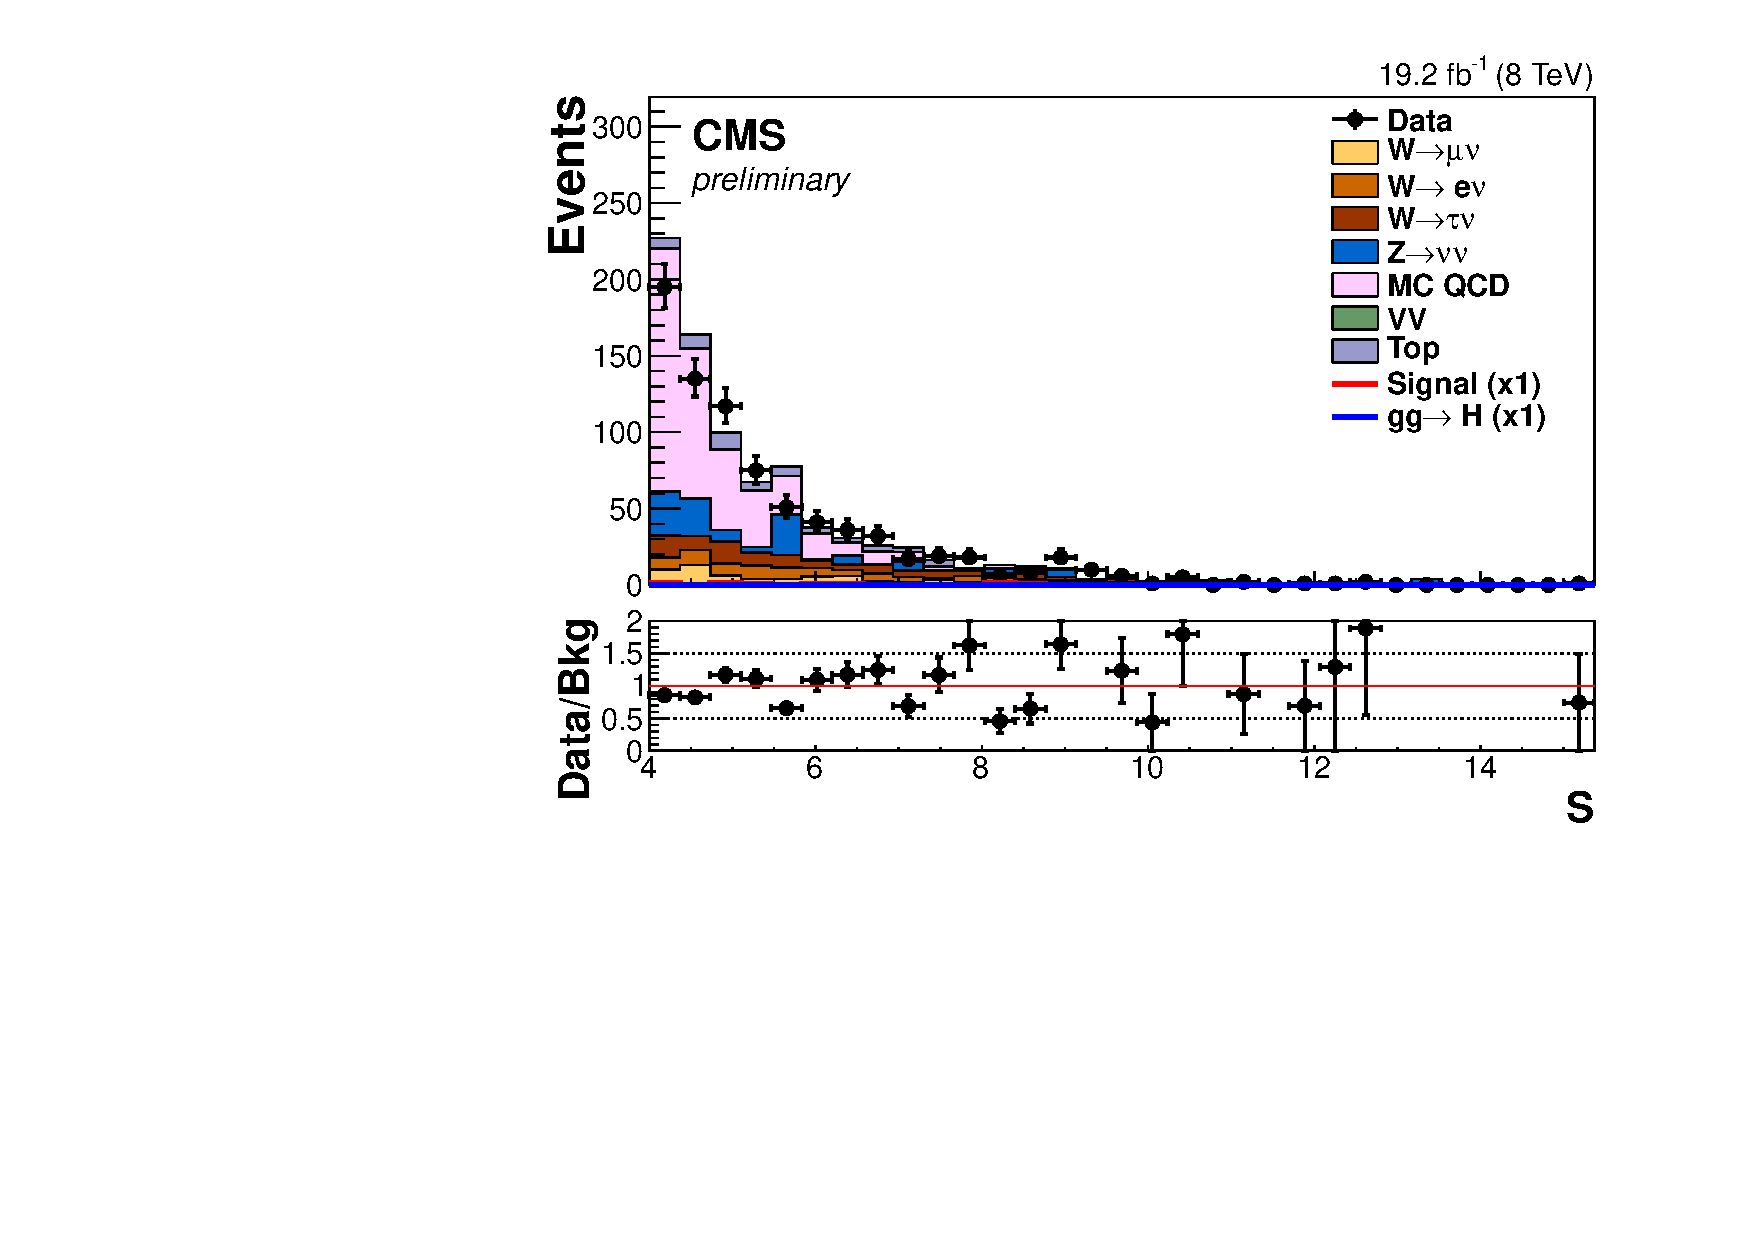
\includegraphics[width=.49\textwidth]{figures/output_invqcd_qcd_metnomu_significance.pdf}
%     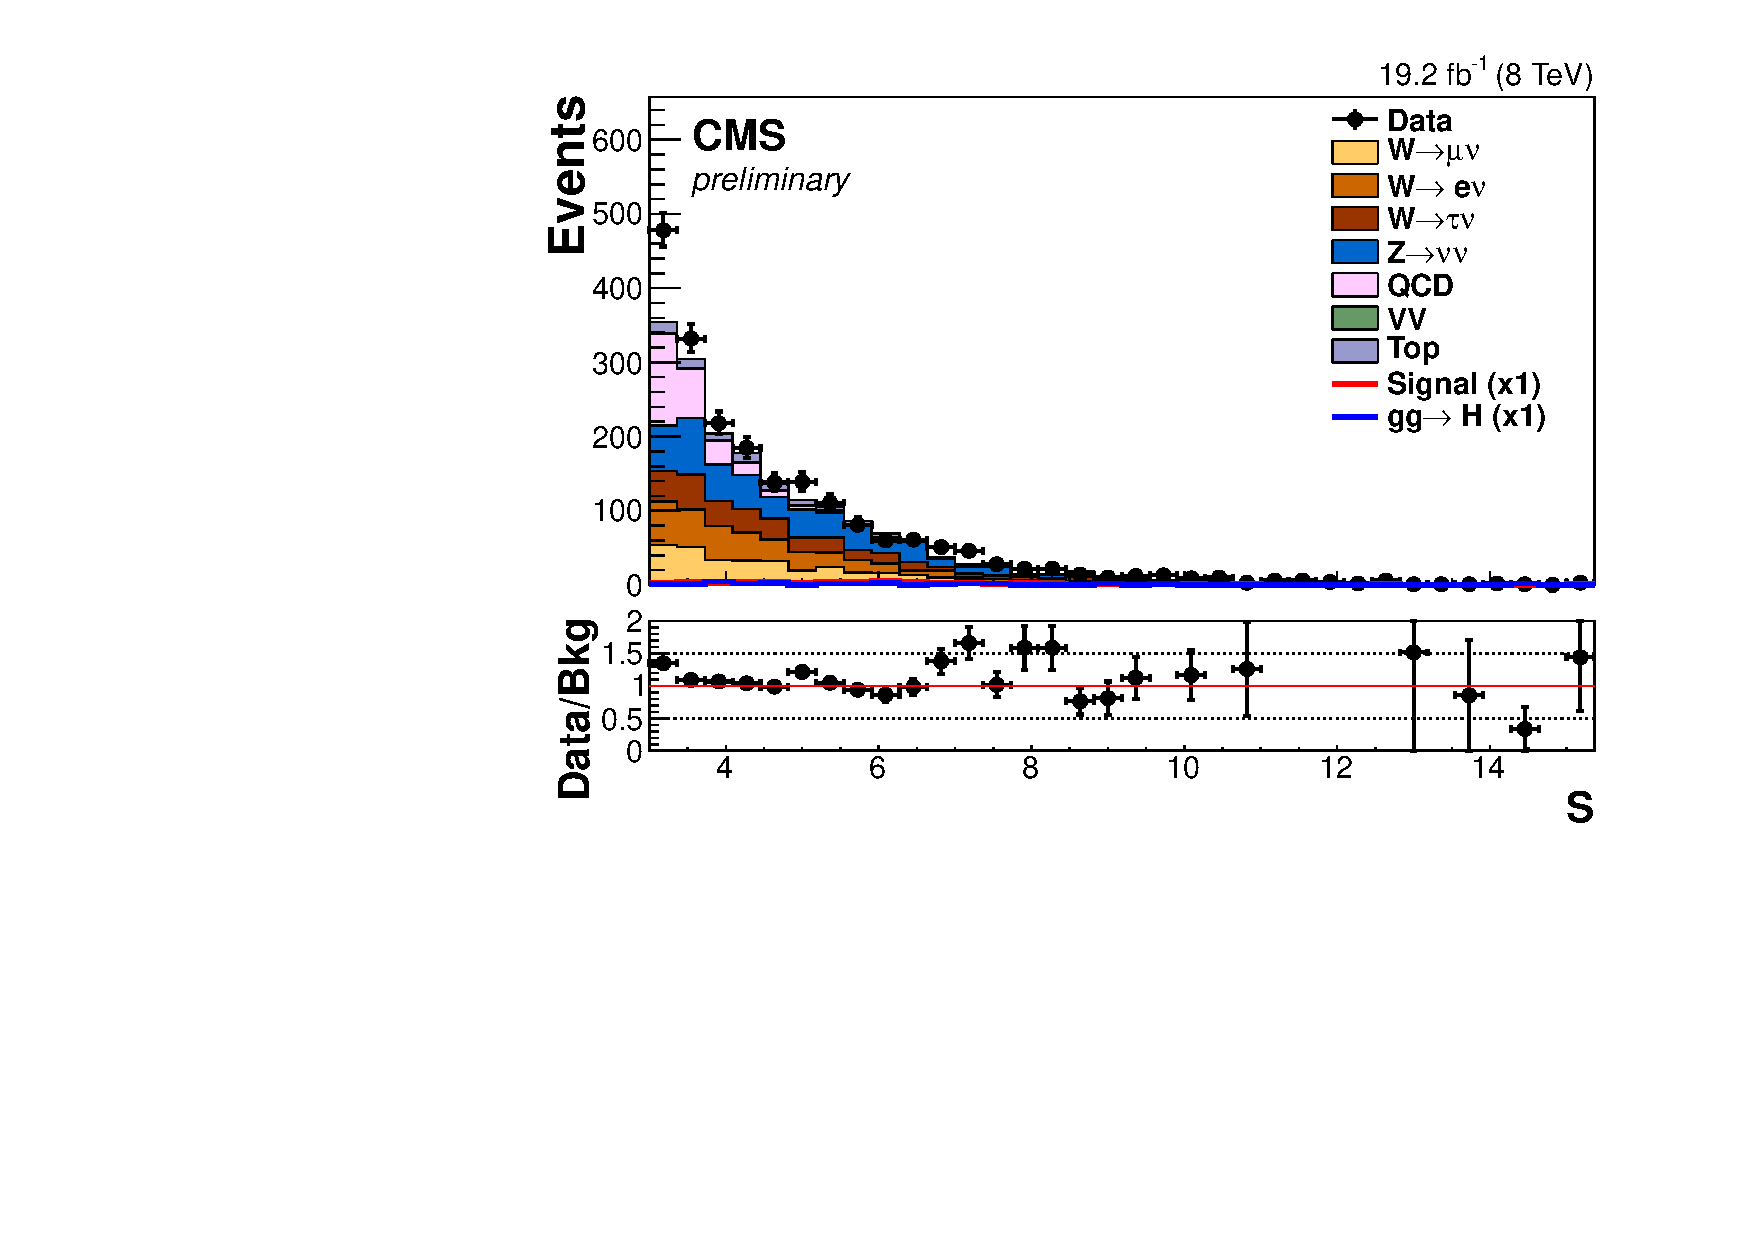
\includegraphics[width=.49\textwidth]{figures/output_invqcd_3j_nunu_metnomu_significance.pdf}
%    \caption{Left: \MET significance \METsig for events with \mindphiall$<1.0$ and
%      \mindphileading$>2.3$. MCQCD is the QCD MC normalised to
%      the background-subtracted data yield. Right: \MET significance \METsig for events
%      with \mindphiall$>1.0$ and at least 3 jets with
%      p$_T>30$\,GeV. The QCD is modelled by data using the inverted
%      \mindphiall$<1.0$ and \mindphileading$>1$ selection, after
%      background subtraction, and normalised to the
%      background-subtracted data yield. In both figures, the W and Z
%      backgrounds have been normalised to their respective control
%      regions in the same conditions. The last bin represents all those events falling above the range of the histogram.}
%     \label{fig:invqcd}
%   \end{center}
% \end{figure}
% 
% 
% A sideband region is used
% to provide a  normalisation of the QCD shape to be used in the signal region. 
% The normalisation sideband is defined as those events in which 
% 3$<$\METsig$<$4 and 1.0$<$\mindphileading$<$2.0.
%  It is observed that the normalisation
% factor decreases rapidly as the requirements on \METsig and \mindphileading
% are tightened. To model this behaviour the normalisation factor is
% measured as a function of the requirement placed on \METsig and
% as a function of the requirement placed on \mindphileading. Both
% functional forms are then extrapolated to the signal region
% requirements. The average of the two extrapolations is used as the central prediction and the envelope is used to assign the systematic uncertainty on the QCD multijets normalisation.
%
%%%%%%%%%%%
%
% \section{Results}
% \label{sec:results}
% The final number of events for each process that passes the selection
% is estimated using the MC in the case of the W, Z and top background
% processes, or the non-isolated \MET events for the QCD multijets
% process, with the normalisation obtained from the control regions, and
% is summarised in Table~\ref{tab:bgSummary}.  The distributions of the
% $\Delta\eta_{jj}$, M$_{jj}$, \METsig and \MET variables, after full selection, are
% shown in Fig.~\ref{fig:sigplots}. An overview of all considered systematic
% uncertainties is given in Table~\ref{tab:syst-qqH}, with the effect on
% the sum of all the background processes and the signal with
% $\mH=125$\GeV and $\BRinv=100$\% given separately.
% 
% \begin{figure}[h!]
%   \begin{center}
%     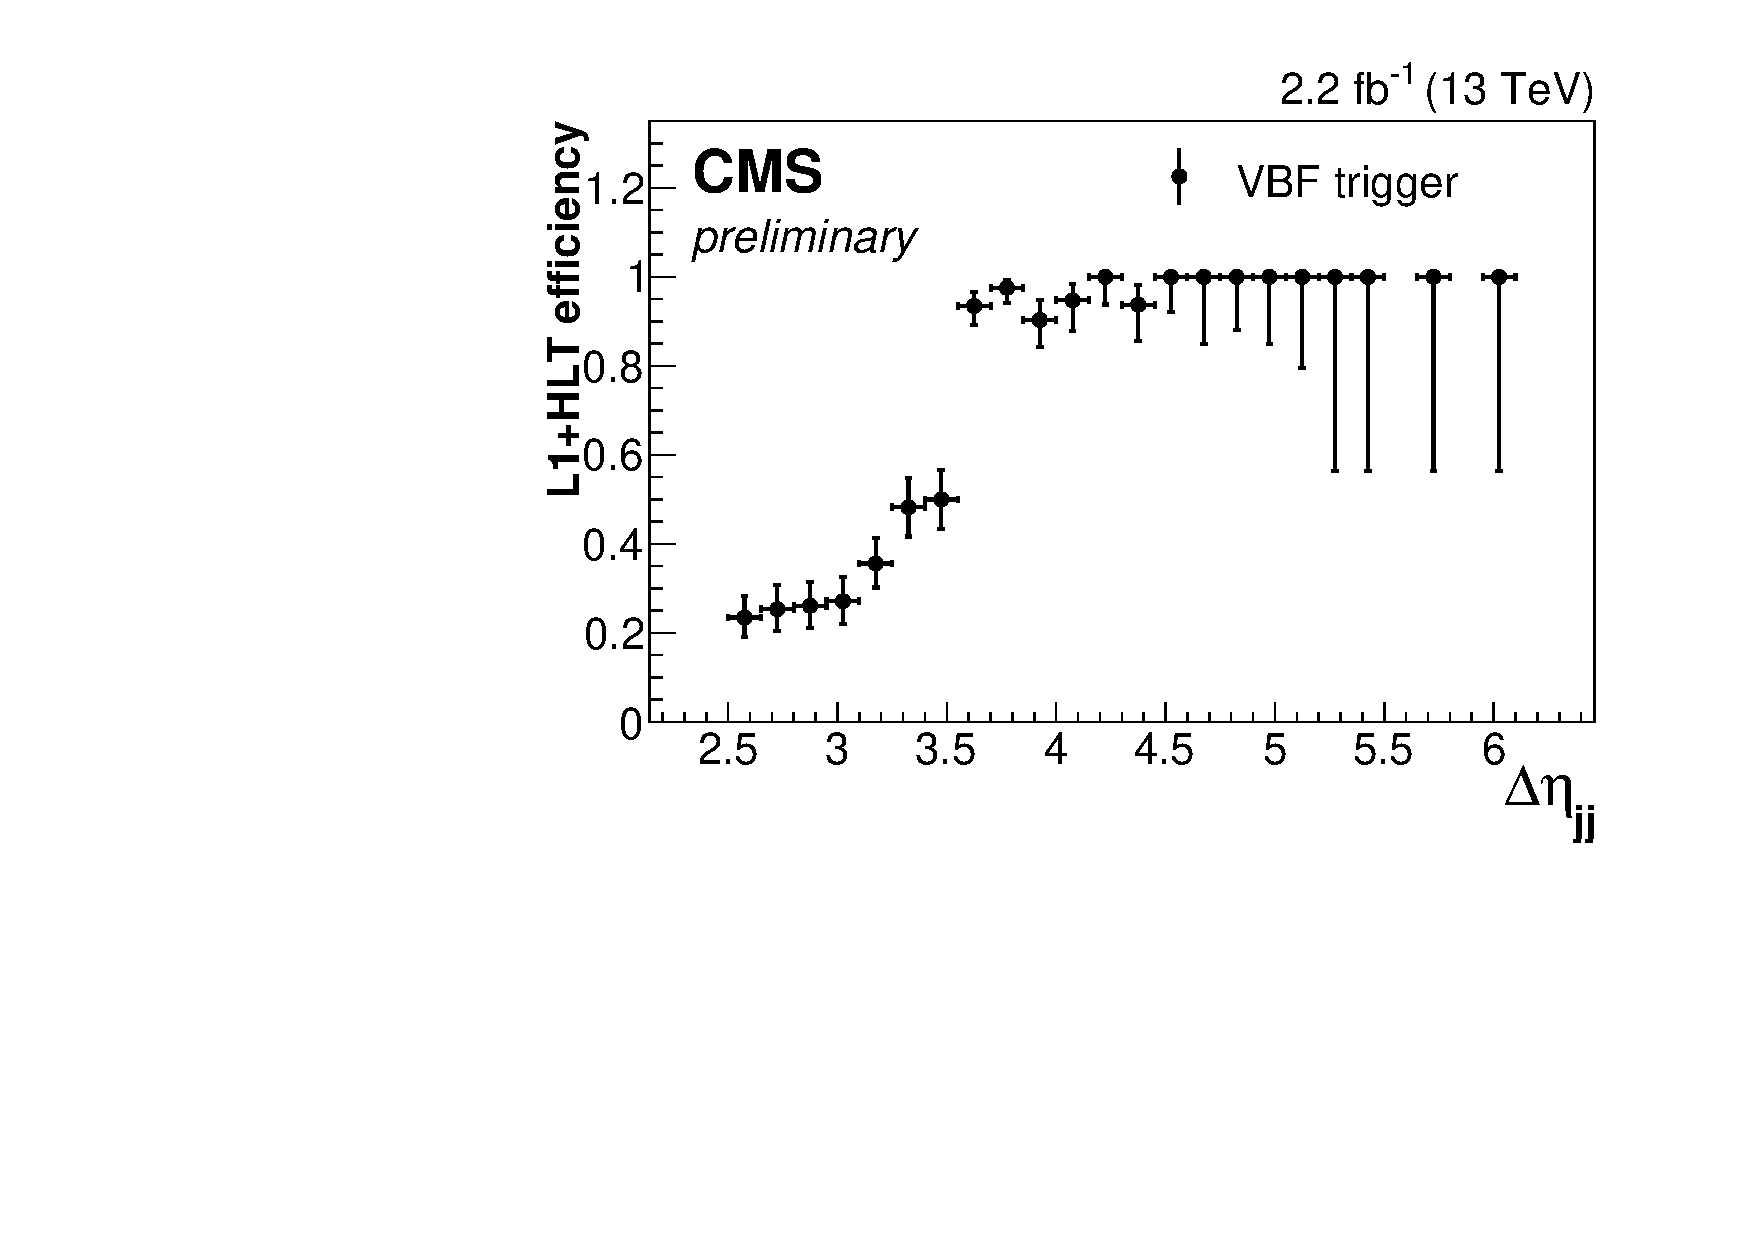
\includegraphics[width=.49\textwidth]{figures/output_sigreg/nunu_dijet_deta.pdf}
%     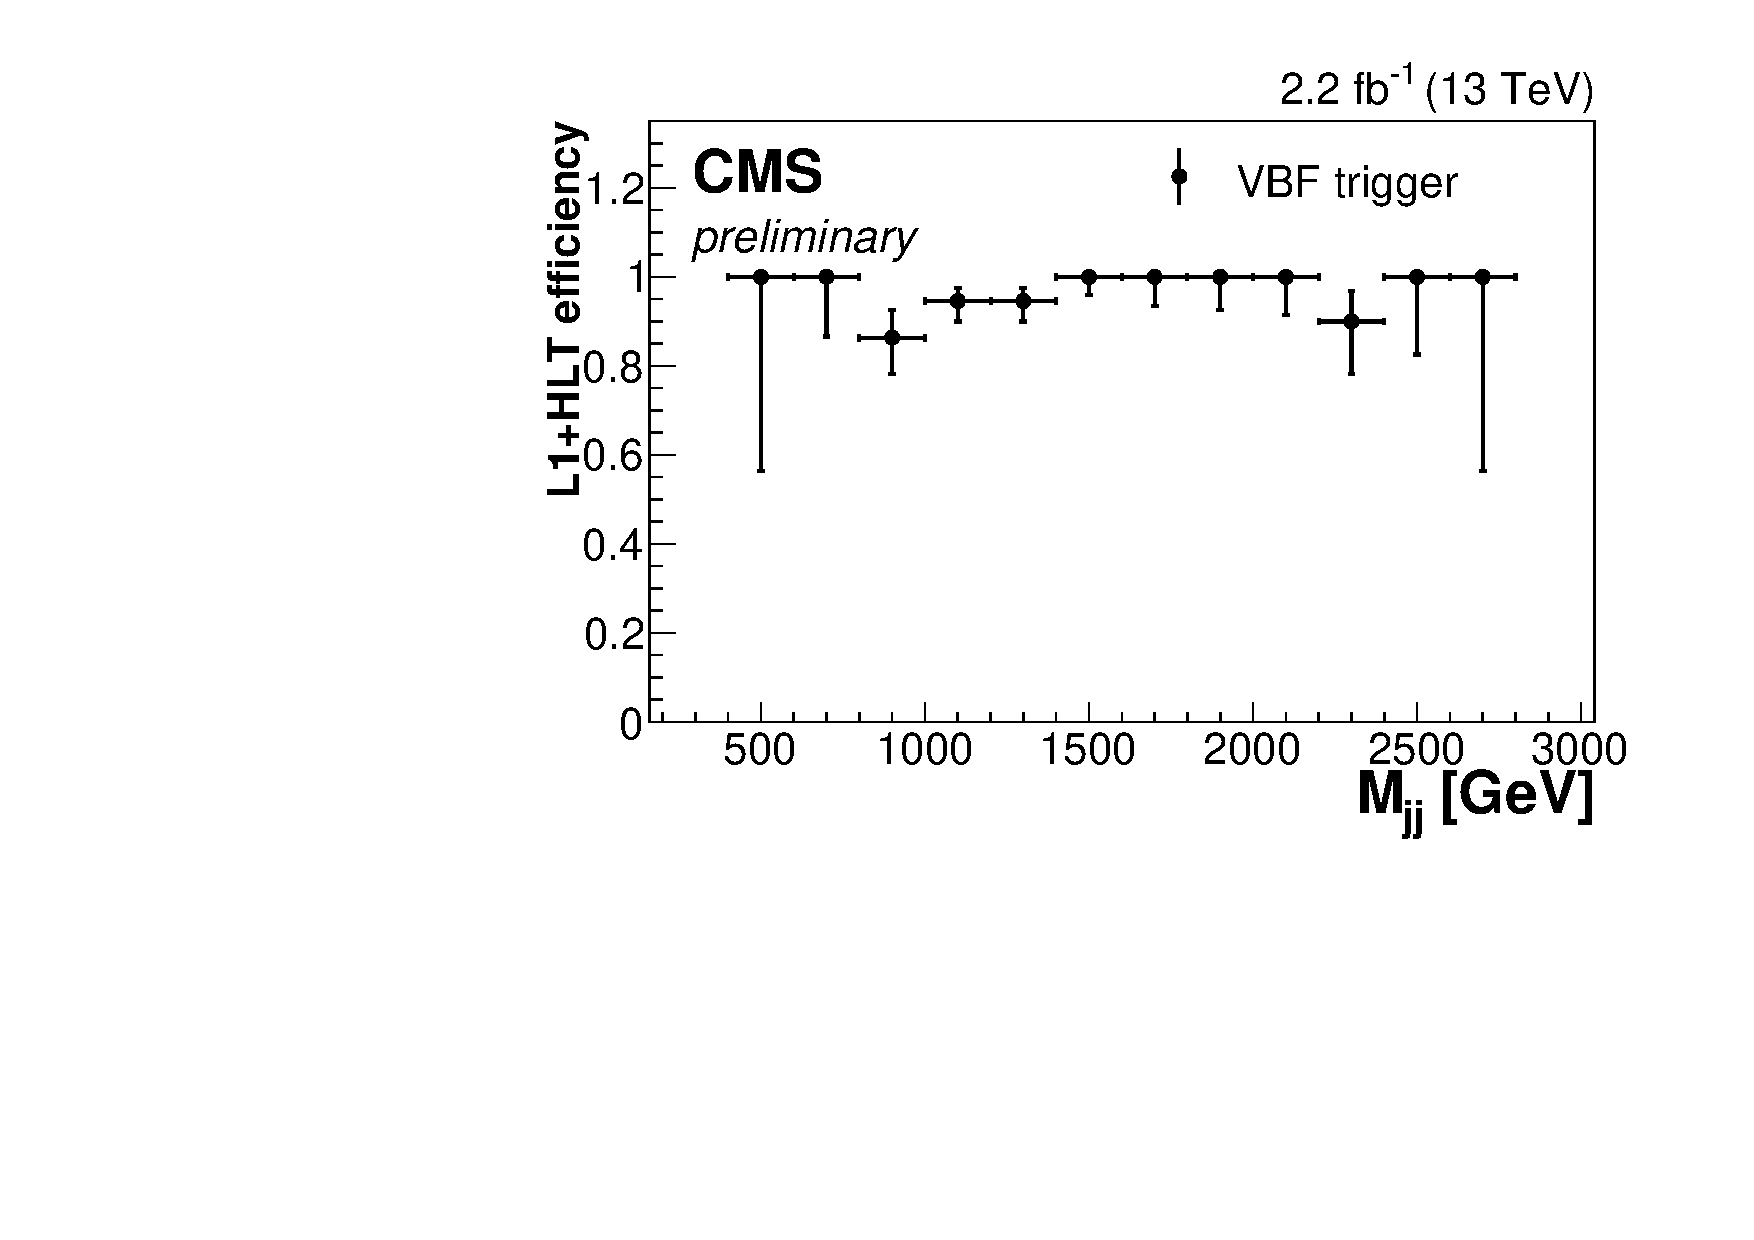
\includegraphics[width=.49\textwidth]{figures/output_sigreg/nunu_dijet_M.pdf}
%     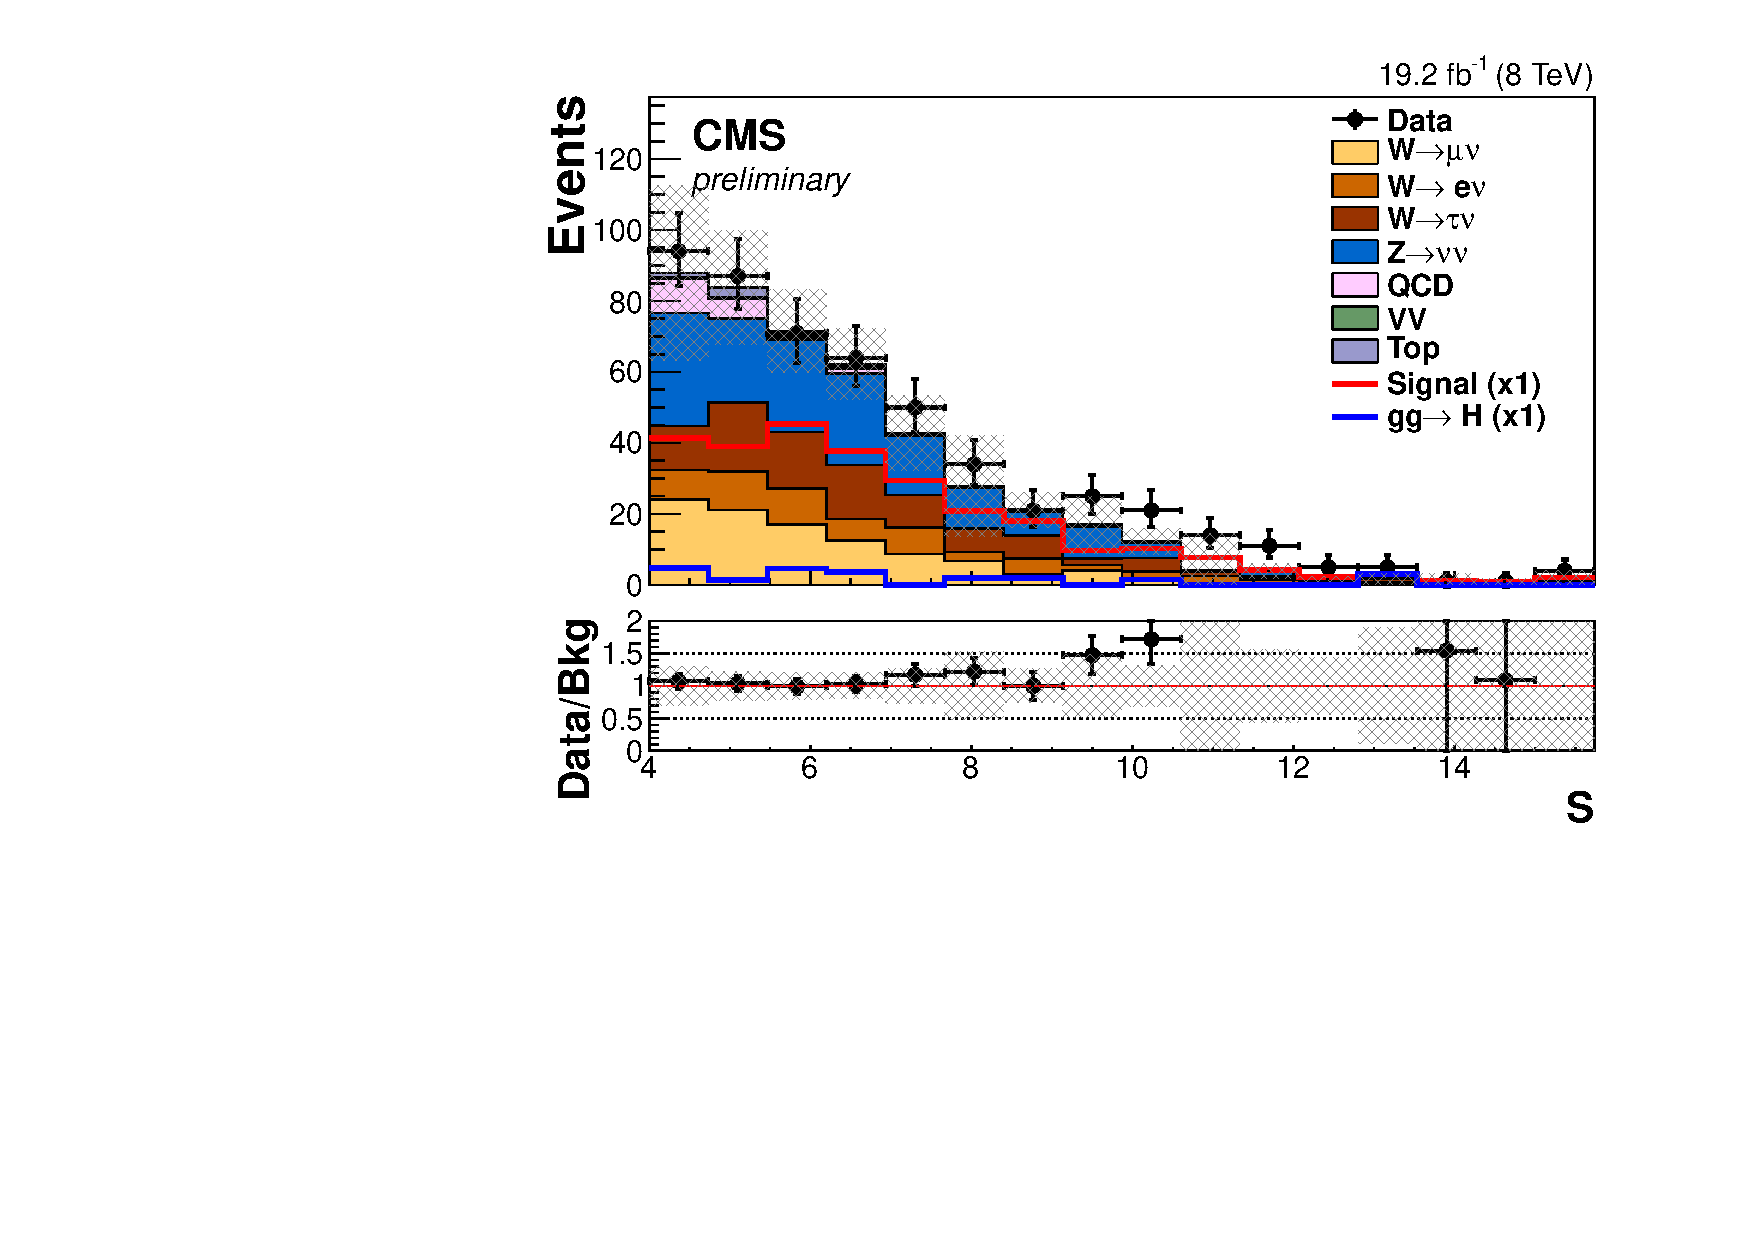
\includegraphics[width=.49\textwidth]{figures/output_sigreg/nunu_metnomu_significance.pdf}
%     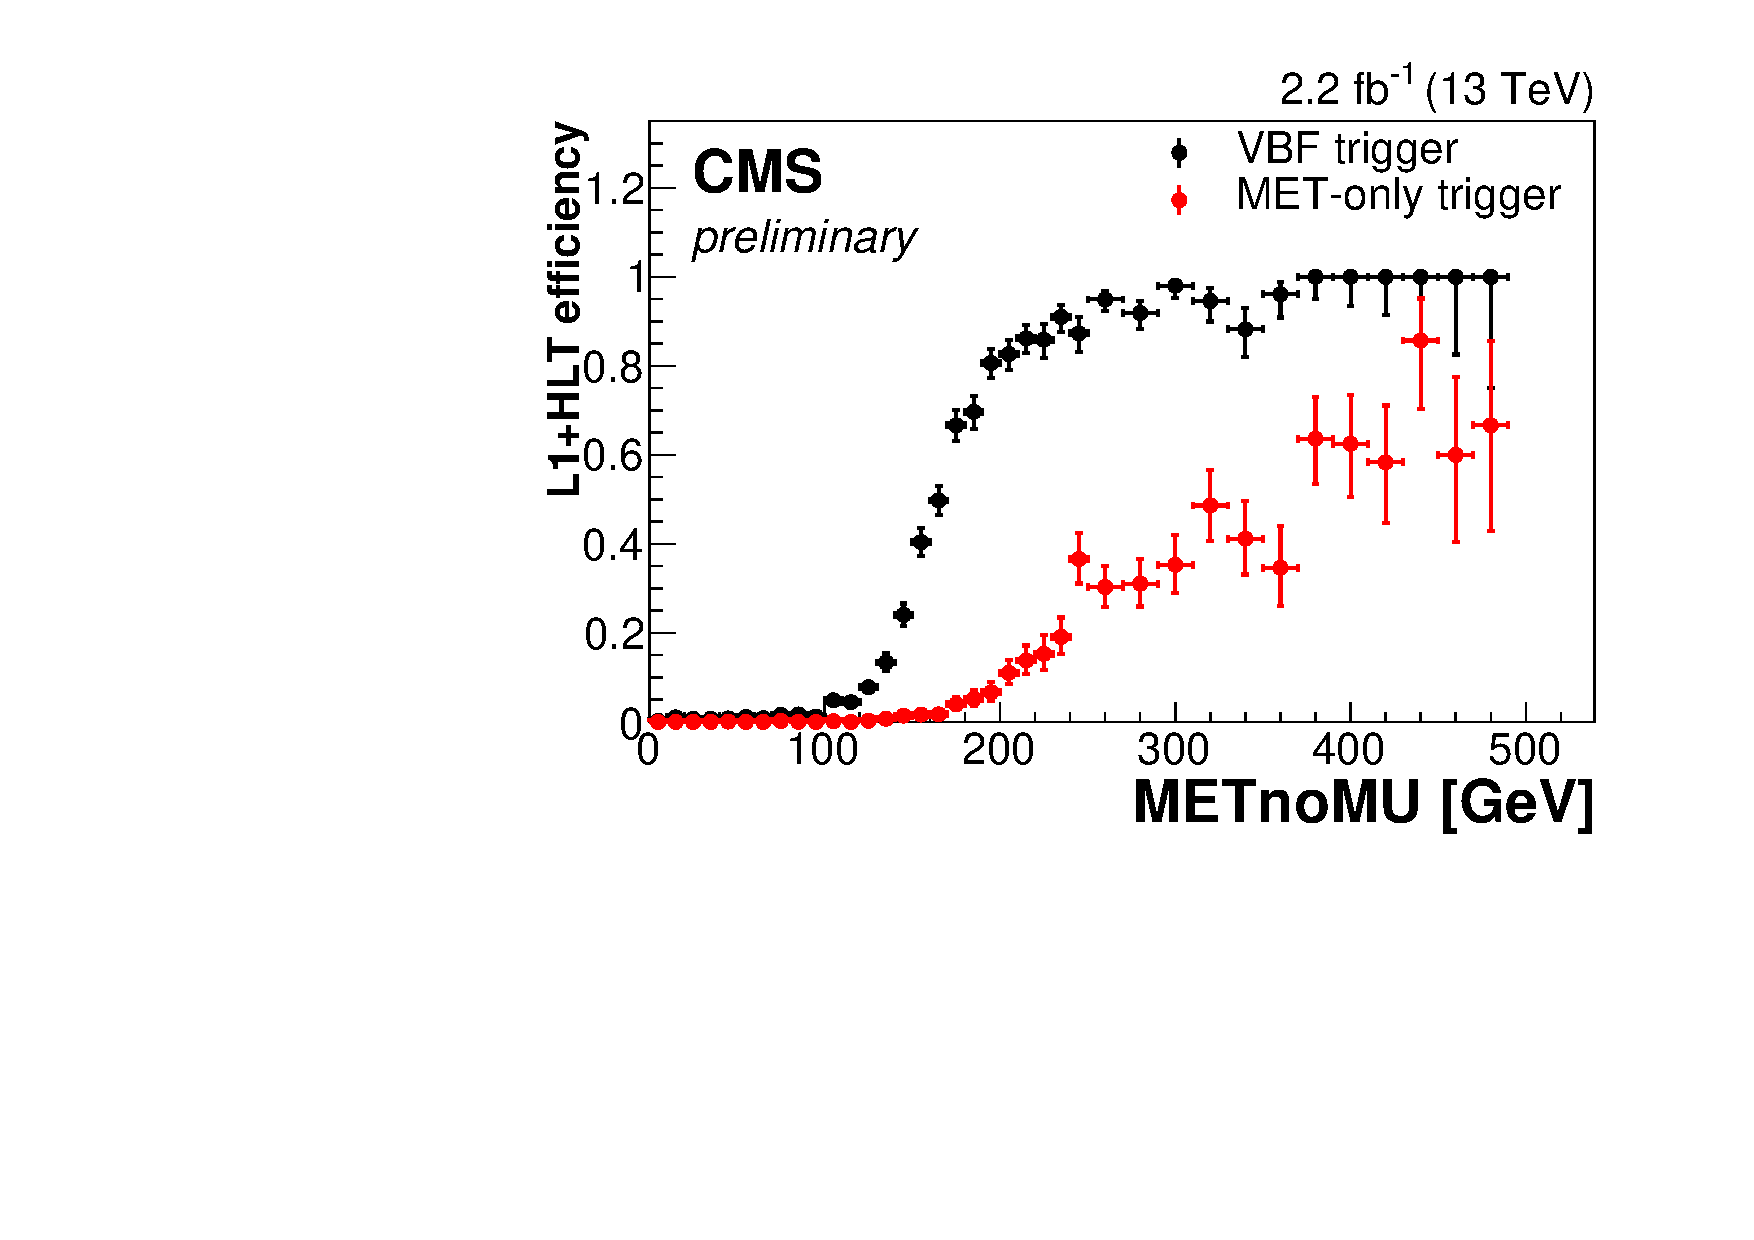
\includegraphics[width=.49\textwidth]{figures/output_sigreg/nunu_metnomuons.pdf}
% 
%     \caption{Top: Pseudorapidity difference between the two VBF tag jets $\Delta\eta_{jj}$ (left), dijet mass $m_{jj}$ (right),  bottom: \MET significance \METsig (left) and \MET (right), in the signal region. The last bin represents all those events falling above the range of the histogram. An excess is seen which is less than 2$\sigma$ in significance as can be seen from the hatched band which indicates the size of the total uncertainty on the background estimate.}
%    \label{fig:sigplots}
%   \end{center}
% \end{figure}
% 
% \begin{table*}[th!]
%         \centering \caption{Summary of the estimated number of
%                 background and signal events, together with the
%                 observed yield, in the VBF search signal region.  The
%                 signal yield is given for $\mH=125$\GeV and
%                 $\BRinv=100$\%. Where two errors quoted they are the statistical and systematic uncertainties respectively, where only one is quoted it is the systematic uncertainty.}  \label{tab:bgSummary}
% \label{tab:res}
% 
% \begin{tabular}{lc}
% \hline \hline
% Process & Event yields \\
% \hline
% $Z\rightarrow\nu\nu$&$158.1 \pm 37.3 \pm 21.2$\\
% $W\rightarrow\mu\nu$&$102.5 \pm 6.2 \pm 11.7$\\
% $W\rightarrow e\nu$&$57.9 \pm 7.4 \pm 7.7$\\
% $W\rightarrow\tau\nu$&$94.6 \pm 13.1 \pm 23.8$\\
% top&$5.5 \pm  1.8$\\
% VV&$3.9 \pm 0.7$\\
% QCD multijet &$17\pm 14$\\
% \hline
% Total Background &$439.4 \pm 40.7 \pm 43.5 $\\
% \hline
% Signal(VBF) &$273.1 \pm 31.2 $\\
% Signal(ggH) &$23.1 \pm 15.9 $\\
% \hline
% Observed data & 508 \\
% \hline \hline
% \end{tabular}
% \end{table*}
% 
% \begin{table*}[h!t]
% \centering
% \topcaption{Summary of the uncertainties on the total background and signal yields. All uncertainties affect the normalization of the yield, and are quoted as the change in \% in the total background or signal estimate, when each systematic effect is varied according to its uncertainties. The signal uncertainties are given for $\mH=125$\GeV and $\BRinv=100$\%.}
% \label{tab:syst-qqH}
% \begin{tabular}{lcc}
% \hline \hline
% Source  & Total background & Signal     \\
% \hline
% Control region data stat. & 9.3 & - \\
% MC stat. & 5.4 & 3.8 \\
% Jet energy scale & 4.6 & 11 \\ 
% $W\rightarrow\tau\nu$ control region extrapolation & 4.3 & - \\ 
% QCD normalisation & 3.2 & - \\ 
% Jet energy resolution & 3.0 & 1.8 \\ 
% Lepton ID efficiency & 2.4 & - \\ 
% Unclustered energy scale & 1.9 & 1.6 \\ 
% Pileup weight & 1.1 & 1.5 \\ 
% Top MC scale factor unc. & 0.25 & - \\ 
% Luminosity & 0.02 & 2.6 \\ 
% QCD scale, PDF and cross section uncertainties & 0.01 & 5.2 \\
% \hline \hline
% \end{tabular}
% \end{table*}
% 
% \section{Limits on the cross section of invisibly decaying Higgs bosons}
% \label{sec:limits}
% Upper limits on the Higgs boson production cross section times \BRinv\,
% are placed at 95\% C.L. using an
% asymptotic CLs method~\cite{Read1,junkcls,Dittmaier:2012vm}, following the
% standard LHC Higgs combination technique~\cite{Chatrchyan:2013lba,HiggsCombination}.
% Systematic uncertainties are treated as nuisance parameters in a frequentist paradigm, as described in~\cite{HiggsCombination},
% and all correlations between processes are taken into account.
% 
% Using this procedure and assuming SM Higgs boson production cross sections and acceptances,
%  the observed (expected) 95\% C.L. limit on \BRinv\,
%  of a SM 125 GeV Higgs boson is 57\% (40\%). The 95\% C.L. limit on %!!MAKE SURE UP TO DATE                                                                   
% \BRinv\, and the 95\% C.L. limit on the cross section times \BRinv, both assuming SM Higgs boson acceptances are
% shown as a function of Higgs boson mass in Fig. \ref{fig:limits}. As can be seen from Table~\ref{tab:syst-qqH} the dominant systematic uncertainty in the analysis is that from the limited numbers of data events in some control regions, in particular the Z control region. If the Z control region statistical uncertainty were to be reduced to the level of that from the $W\rightarrow\mu\nu$ control region the expected 95\% C.L. limit on the cross section times \BRinv for a SM 125 GeV Higgs boson would be reduced to 33\%.
% 
% The result is also combined with that obtained by CMS in searches in the channel where the Higgs boson is produced in association with a Z which was reported in ~\cite{Chatrchyan:2014tja}. The procedure for this combination is also described in ~\cite{Chatrchyan:2014tja}. The 95\% C.L. observed (expected) limit on \BRinv\, after combination is 47\% (35\%) for a SM 125 GeV Higgs boson.
% 
% \begin{figure}[h!]
%   \begin{center}
%     \includegraphics[width=0.49\textwidth]{figures/vbflimit.pdf} %!!UNBLIND ALREADY IN                                                                       
%     \includegraphics[width=0.49\textwidth]{figures/vbfxslimit.pdf}
%  \caption{The 95\% C.L. limit on \BRinv\, of a SM Higgs
% boson (\cmsLeft) and the 95\% C.L. limit on the cross section times
% \BRinv\, (\cmsRight)as a function of the Higgs
% boson mass, assuming SM Higgs boson acceptances.}
%     \label{fig:limits}
%   \end{center}
% \end{figure}




